\documentclass[a4paper]{article}
%% Language and font encodings
\usepackage[english]{babel}
\usepackage[utf8x]{inputenc} \usepackage[T1]{fontenc}
\usepackage{amsfonts}
\usepackage{graphicx}
\usepackage{amssymb}
\usepackage{bm}
\usepackage{amsmath}
\usepackage[colorlinks=true, allcolors=blue]{hyperref}
\usepackage{titlesec}
\usepackage{wrapfig,setspace,subfig}
\usepackage[labelfont={bf,it}, textfont=it, justification=centering]{caption}
%% Sets page size and margins
\usepackage[
	a4paper,
	top=3cm,
	bottom=2cm,
	left=3cm,
	right=3cm,
	marginparwidth=1.75cm
]{geometry}

%commands
\newcommand{\mat}[1]{\mathbf{#1}}
\newcommand{\vect}[1]{\bm{#1}}
\newcommand{\com}[1]{}

%\setlength{\parindent}{0em}
%\setlength{\parskip}{8pt}

%\titlespacing\section{0pt}{12pt}{2pt}
%\titlespacing\subsection{0pt}{12pt}{2pt}

\title{$\vec{E}$mission}
\author{2137402D, 2200581K, 2228029M, 2176989S, 2206189S}
\begin{document}
\maketitle

\begin{abstract}
The Laplace equation is one of the cornerstones of classical electrostatics. 
In this report we will examine different numerical methods which may be used to 
obtain numerical estimations to 2-dimensional problems where the geometry is 
too complex for analytical manipulation. Specifically, we employed iterative 
methods of Successive Over Relaxation (SOR) as well as direct methods which 
utilise the LU-decomposition algorithm. We then compared the two methods for 
problems of existing analytical solutions as well as those demanding numerical 
simulation, conducting both error and performance analysis. Parallel to this, a 
GUI was developed to encapsulate the project into a single executable, allowing 
for user defined geometry and charge generated from dynamic drawing.
\end{abstract}

\section{Introduction}
We initially solved two problems mathematically in order to have some 
analytical solutions which could be used to reconcile with the results that our 
numerical approximations might come up with. The two problems are illustrated 
and enumerated below:
\begin{figure}[h]
\centering
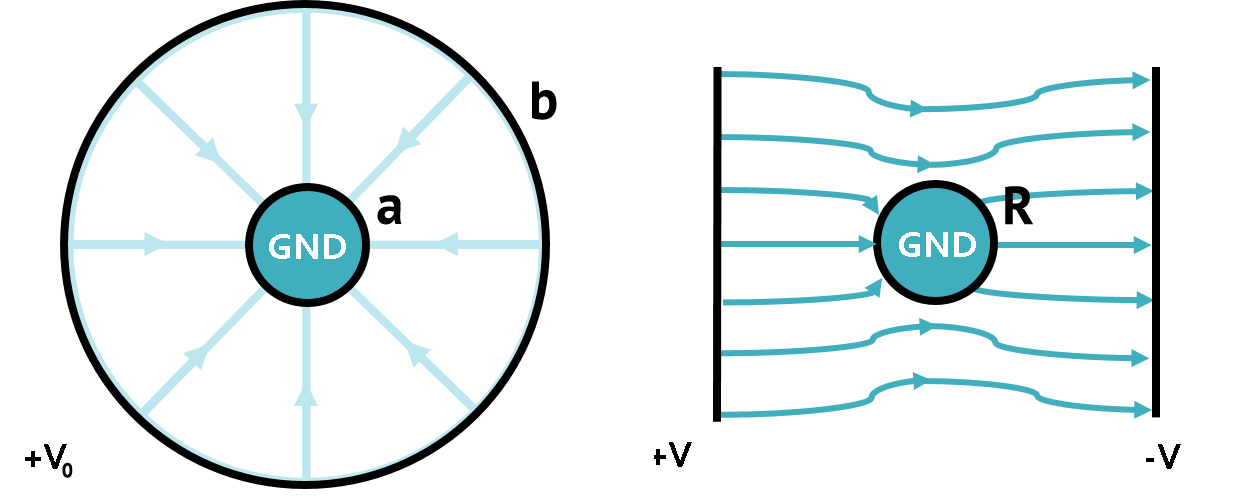
\includegraphics[width=0.7\textwidth]{AnalProblems.png}
\caption{\label{fig:frog}Problem 0 (radii a, b) and Problem 1 (radius R)}
\end{figure}

\section{Analytical problems}
To solve problem 0 we need to begin from the expression of Laplace's equation 
in cylindrical coordinates, where as usual, $r$ is the radial distance, $\phi$
is the angular coordinate and $z$ the height:
\begin{equation} \label{laplacefull}
\nabla^2V=\frac{1}{r}\frac{\partial}{\partial r}\Big( \frac{r\partial 
V}{\partial r} \Big) + \frac{1}{r^2}\frac{\partial^2V}{\partial\phi^2} + 
\frac{\partial^2V}{\partial z^2} = 0 
\end{equation} 
Firstly, we identified that there is circular geometry, so we could omit the 
angular coordinate, as well as disregard the height, thus reducing the problem 
to 1-dimensional geometry, described by the truncation of equation 
\ref{laplacefull} seen underneath.
\begin{equation}\nabla^2V=\frac{1}{r}\frac{\partial}{\partial r}\Big( 
\frac{r\partial V}{\partial r} \Big) = 0
\end{equation}
Solving this equation for $V$ is relatively easy, and integrating twice will 
suffice.
\begin{equation}\int\frac{1}{r}\frac{\partial}{\partial r}( \frac{r\partial 
V}{\partial r} )dr = \int0dr \implies r\frac{\partial V}{\partial r} = constant 
= c
\end{equation}
\begin{equation}\implies \int\frac{\partial V}{\partial r}dr = \int \frac{c}{r} 
dr \implies V(r) = c\ln(r) + d
\end{equation}
Finally, using our boundary conditions $ V(a) = 0$ and $V(b) = V_0$ we obtained 
an equation governing the potential field:
\begin{equation}\boxed{V(r) = \frac{V_0}{k}\ln\Big(\frac{r}{a}\Big) \textrm{ 
where k} = \ln\Big(\frac{b}{a}\Big) }\end{equation}
We then proceeded to solve problem 1, which posed a more interesting challenge. 
Due to this problem's geometry, only the height variable can be omitted and 
both the remaining variables in equation \ref{laplacefull} needed to be 
considered as seen underneath. 
\begin{equation}\nabla^2V=\frac{1}{r}\frac{\partial}{\partial r}\Big( 
\frac{r\partial V}{\partial r} \Big) + 
\frac{1}{r^2}\frac{\partial^2V}{\partial\phi^2} = 0\end{equation}
This particular equation has solutions of the form:
\begin{equation} \label{gensol}
(r,\phi)=\sum_{n=1}^{\infty} (C_nr^n+\frac{D_n}{r^n})(A_n 
\cos(n\phi)+B_n\sin(n\phi)) 
\end{equation}
We obtained this by assuming separation of variables $V(r) = Q(\phi)P(r)$ such 
that
\begin{equation}\nabla^2V=\frac{1}{r}\frac{\partial}{\partial r}\Big( \frac{rQ 
\partial P}{\partial r} \Big) + 
\frac{1}{r^2}P\frac{\partial^2Q}{\partial\phi^2} = 0
\end{equation}

\begin{equation}\implies \frac{Q}{r}\bigg(\frac{\partial P}{\partial 
r}+r\frac{\partial^2P}{\partial r^2}\bigg) + 
\frac{1}{r^2}P\frac{\partial^2Q}{\partial \phi} = 0
\end{equation}
Multiplying both sides by $\frac{r^2}{QP}$ and reordering yields
\begin{equation}\frac{r^2}{P} \frac{\partial^2P}{\partial r^2} + \frac{r}{P} 
\frac{\partial P}{\partial r} = - \frac{1}{Q} \frac{\partial^2Q}{\partial 
\phi^2} = n^2 \end{equation}
for some constant n. The part with Q$(\phi)$ can be solved through considering 
the auxiliary equation which yields imaginary roots, thus obtaining solutions 
of the form:
\begin{equation} \label{sol1}
Q(\phi) = (A_n\cos(n\phi)+B_nsin(n\phi))
\end{equation}
with the restriction that $n\in \mathbb{Z}$ because of the single-valuedeness 
of Q($\phi$), which means that $Q(\phi) = Q(\phi+2\pi)$, corresponding to a 
full rotation around the conductor, leading to a behaviour of $cos(n\phi)) = 
cos(n\phi + 2n\pi)$ which in turn restricts n to be an integer.

The part with $P(r)$ is called a radial equation where we notice that the order 
of differentiation associated with each term is equal to the power of each r 
term, implying that a solution of the form $P(k) = r^k$ would suffice, given 
the exception that $k \neq 0$. Attempting such an approach gives
\begin{equation}r^2\frac{\partial^2r^k}{\partial r^2}+r\frac{\partial 
r^k}{\partial r} = n^2r^k \end{equation}
\begin{equation}\implies r^2k\frac{\partial^2r^{k-1}}{\partial r^2}+rkr^{k-1} = 
n^2r^k \end{equation}
\begin{equation}\implies r^2k(k-1)r^{k-2} + rkr^{k-1} = n^2r^k \end{equation}
\begin{equation}\implies k^2 - k + k = n^2\end{equation}
\begin{equation}\implies k = \pm n
\end{equation}
This means that by using the Principle of Superposition we obtain solutions of 
the form 
\begin{equation}\label{sol2}
P(r)=C_nr^n + D_nr^{-n}
\end{equation} 
Combining the two forms found in equations \ref{sol1} and \ref{sol2} we deduce 
the general solution quoted initially in equation \ref{gensol} which can be 
used to solve our geometry.

Now we will examine the physics of the problem. It is safe to assume that for a 
radial distance $r$ much larger than the radius of the conductor $R$ then the 
potential and electric fields would behave as if unaffected by the presence of 
the conductor, i.e. the equation describing the potential field at $r\ll R$ is 
$V(r,\phi) = -E_0 r\cos(\phi) + K$ where $E_0$ is how the strength of the 
electric field relative to the distance travelled from some point and $K$ is a
constant of integration. Therefore, by comparing with the form of equation
\ref{gensol} we can identify that for this to be matched, n should equal 1 and
the $\sin(n\phi)$ term should be omitted. We can then denote the remaining
multiplied constants as $C = C_1A_1$ and $D=D_1A_1$ for simplicity, arriving at
\begin{equation}V(r,\phi) = Dr\cos(\phi) + \frac{C}{r}\cos(\phi) = -E_0 
r\cos(\phi) + K
\end{equation}
From the general solution and the behaviour of V at large radial distances 
respectively. It is then easy to see that $D = -E_0$. Finally we consider our 
boundary conditions at the surface of the conductor, $r = R$ where we know that
\begin{equation}V(R,\phi) = -E_0R\cos(\phi) \frac{D}{R}\cos(\phi) = 0 
\end{equation}
\begin{equation}\implies D = E_0R^2\end{equation}
\begin{equation}\implies \boxed{V(r,\phi) = -E_0 
\bigg(r-\frac{R^2}{r}\bigg)\cos(\phi)}\end{equation}
It's now easy to compute $\vec{E}$ from the definition of the cylindrical gradient
\begin{equation}\implies \boxed{\vec{E}(r,\phi) = 
E_0\bigg[\hat{r}\bigg(1+\frac{R^2}{r^2}\bigg)\cos(\phi) - 
\hat{\phi}\Big(1-\frac{R^2}{r^2}\Big)\sin(\phi)\bigg]}\end{equation}
Finally, to make a sanity check we can compute the charge density on the 
conductor's surface.
Giving us that the total charge density is zero as we would expect.
As mentioned earlier these analytical solutions were obtained in order to 
provide values which the code we developed could be compared with. The main 
problem that interested us was the geometry of a multi-wire proportional 
chamber which can be seen underneath. 

\begin{figure}[h]
\centering
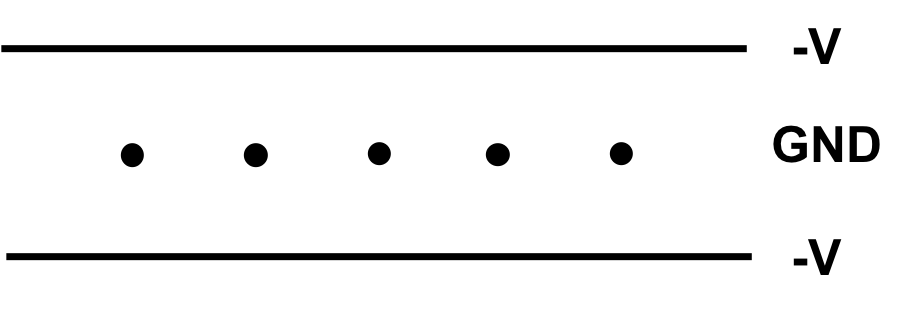
\includegraphics[width=0.7\textwidth]{NobelProblem.png}
\caption{\label{fig:frog}A cross section of the multi-wire proportional chamber 
(MWPC)}
\end{figure}

\section{Preparation for Numerical Analysis}
The multi-wire proportional chamber was developed by George Charpak in 1968. As 
seen in the above image the MWPC consists of wires at ground potential, 
enclosed in a chamber at negative potential such that any negatively charged 
particles like electrons are drawn towards the wires due to the electric field. 
This effect is amplified because the chamber is filled with a gas that becomes 
ionised by incoming charged particles. The electric field then accelerates the 
ions and electrons which in turn create more ionisations which are drawn 
towards the array of wires, registered as a charge. This effect, known as 
Townsend avalanche is proportional to the ionisation effect of the incoming 
particle which means that by combining information from the wires, the 
particle's trajectory may be determined. This method increased the rate of 
detection by a factor of 500 compared to the bubble chambers used earlier and 
resulted in George Charpak being awarded the Nobel Prize in Physics in 1992. 
Inventions like this further fortify our interest in modelling potential 
fields.

An analytical solution does not exist for such a geometry so we resorted to 
applying numerical techniques on the Laplace equation. This was done by 
considering a truncation of the Taylor expansion, for small distance $h$ travelled 
in the $x$ and $y$ directions.
\begin{equation}V(x\pm h,y) = V(x,y)\pm h\frac{\partial V(x,y)}{\partial x} + 
h^2 \frac{\partial^2V(x,y)}{\partial x^2} \pm h^3 
\frac{\partial^3V(x,y)}{\partial x^3}+ O(h^4) \end{equation}
\begin{equation} V(x,y\pm h) = V(x,y)\pm h\frac{\partial V(x,y)}{\partial y} + 
h^2 \frac{\partial^2V(x,y)}{\partial y^2} \pm h^3 
\frac{\partial^3V(x,y)}{\partial y^3} + O(h^4) \end{equation}
\begin{equation} \label{FPS} \implies V(x+h,y)+V(x-h,y)+V(x,y+h)+V(x,y-h) = 
4V(x,y)+O(h^4)\end{equation}
since the terms of $h$ and $h^3$ cancel out due to their signs and the terms of 
$h^2$ are equal to zero in the case of the Laplacian in free space. This is the 
quintessential equation to this project and it informs us that the value of the 
potential at some point in our 2-dimensional grid is approximately equal to the 
mean of the 4 surrounding points, hence its name `the five point star (FPS)'.\\

At this instance the team split into 3 subgroups with the aim of creating a 
program with a GUI where the user could enter any desired geometry and charge, 
with the code approximating the potential field using the FPS. The first 
subgroup was tasked with developing an iterative solution to the FPS, the 
second a direct solution to the FPS and the third a working GUI which could 
encompass all aspects of the code including the drawing and plotting phase. 
All of the inner workings will be elucidated further in this report.
The first problem we faced after compartmentalising the work was how could the 
user set the charge of the drawn shapes and furthermore how could the code 
convey the presence of shapes and their charge to the numerical methods 
mentioned above. To that extend we came up with a simple and aesthetically 
appealing solution, where the charge was related to a colour gradient. The user 
first specifies the maximum voltage which he is interested in and that is then 
associated with a colour gradient, where positive charge relates to red and 
negative to green. Any undefined space remains white and ground charged shapes 
are black.

After the user has finished drawing the shapes and requests for a computation 
of the potential field we read the resulting image as a PNG and then pick out 
information pixel by pixel. Running the algorithm in reverse we can deduce the 
charge at each pixel from its colour as well as if it is a defined shape of 
constant charge or empty space (i.e. if it is white) and store this information 
in a matrix. This means that for an image of N$\times$N pixels the code is
supplied with a 3-dimensional array of $N\times N \times 2$ dimensions since
every pixel corresponds to 2 values, the first one being the amount of charge,
and the second one conveying whether that pixel corresponds to a shape or
not.  

%%%%%%%%%%%%%%%%%%%%%%%%%%%%%%%%%%%%%%%%%%%%%%%%%%%%%%%%%%%%%%%%%%%%%%%%%%%%%%%
%%%%%%%%%%%%%%%%%%%%%%%%%%%%%% PART 2 SID %%%%%%%%%%%%%%%%%%%%%%%%%%%%%%%%%%%%%
%%%%%%%%%%%%%%%%%%%%%%%%%%%%%%%%%%%%%%%%%%%%%%%%%%%%%%%%%%%%%%%%%%%%%%%%%%%%%%%

\section{Introduction to the Direct Method}
The direct method is possibly the most logically straightforward way to solve
for the values of the mesh points. It involves expressing the relationships of
the various grid points with each other through a system of simultaneous
equations, and then solving this system to obtain a vector containing the
solutions to the mesh points. Thus, in contrast to the iterative methods,
results are obtained at their final accuracy rather than being successively
improved over several cycles.

In our implementation we consider as system of the form:
\begin{align*}
	-4&V_1+V_2+0V_3+0V_4+V_5+\dots+0V_{16}&=0\\
	&V_1-4V_2+V_3+0V_4+0V_5+V_6+\dots+0V_{16}&=0\\
	&\vdots\\
	0&V_1+\dots+V_{12}+0V_{13}+0V_{14}+V_{15}-4V_{16}&=0\\
\end{align*}
Which can be expressed by the matrix equation:
\begin{equation}
	\mat{A}\vect{v}=\vect{b}
	\label{matEq}
\end{equation}
Where $\mat{A}$ is a matrix holding the coefficients of the system, $\vect{v}$
holds the voltage solutions, and $\vect{b}$ represents the right hand values of
the system. We could now apply a variety of generic matrix solving techniques
to find $\vect{v}$ but these methods quickly become impossible to practically
implement in larger problems for reasons discussed in the following sections.

\section{Implementation of the Direct Method}
The first thing to notice is that if we have a $N\times N$ grid then the
coefficient matrix has $N^4$ elements. This quartic growth means that the
storage space required quickly overtakes any realistic memory capacity.
Furthermore, even if one could procure such an expansive memory device, we
would still leave much to be desired in terms of efficiency. To understand why
this is, consider the structure of the matrix $\mat{A}$. We can notice that on
any given line there are at most five non zero elements: the point of interest,
and the four points around it. The rest of the elements on that row are
initialised to zero. The net effect of this is that the matrix $\mat{A}$ is
\emph{extremely} sparse, especially for large $N$. In fact the sparseness of
the matrix is the principle factor on which optimisations are made~\cite{NR}.
In the next section we discuss methods of storing large sparse matrices and the
challenges they present.

\subsection{Storage Systems for Sparse Matrices}
The essential idea behind sparse matrix compression is to minimise the required
storage space by only storing non-zero elements and their respective positions
such that all the information of the original matrix is still preserved.
Although there are several compression schemes available~\cite{101matstore} we
utilised coordinate storage (COO) and compressed column storage (CCS).

The COO storage format is possibly the simplest to understand and implement. It
essentially involves storing three columns or arrays of data: one that tracks
the row numbers of the non-zero elements, another that tracks the column
numbers, and finally one that tracks the values themselves. While this method
offers a fairly good compression rate for large $N$ and is easy to implement,
it does suffer from a few drawbacks. Firstly, it does not optimise on the fact
that several non-zero elements share the same column (or row) number; secondly,
and more significantly, if we wanted to access the non-zero element $v$ with
row number \texttt{i} and column number \texttt{j} we would have to scan
through all the elements preceding it.

To overcome these shortfalls we may use the CCS format. As done previously we
will maintain three data sets, one of which will hold the non-zero values. The
second data set will hold the corresponding row values of those elements.
Finally, the third set holds holds \emph{column offsets} which tell us where in
the value set the next column begins. This not only reduces the space required
but also allows us to \emph{jump} to a requested value by referring to the
column offsets rather than scanning through every element~\cite{101matstore}.

In our code we write in the COO format and use the package
CSPARSE~\cite{csparse} to convert this into the CCS format before solving.

\subsection{Formulating the Linear System}
The system of equations as described thus far holds no information with regard
to any specific geometry and therefore solves no particular problem. Thus, an
essential step is finding a mechanism whereby the system can be tweaked to
reflect a given problem.

To see how this was achieved, consider the $4 \times 4$ grid shown
in Fig.~\ref{gridFig} with a voltage of 25V at $v_6$. How can this information
be represented in the system? The solution employed was to zero out the row
corresponding to $V_6$ (row 7 if we index from 0) and write a 1 into its
diagonal. We then write 25 in the corresponding element of the $\vect{b}$
vector. The reason this works can be seen by multiplying out the left hand side
of~\eqref{matEq}. Notice that all the zero elements in row 7 will ensure almost
all the variables disappear, leaving only the 1 in the diagonal to be
multiplied to yield the equation $v_6=25$ which is precisely the restriction we
wished to specify.

To deal with the boundaries we use a method we shall call \emph{adaptive
stencilling}\footnote{this is a fairly simple modification of the five point
star, but at the time of writing we failed to find reference or utilisation of
it in the scientific literature}. The idea is to adapt the number of
\emph{legs} of our stencil as we crawl the mesh depending on where we are;
changing from a three point stencil to a four point one when we are at the
corners or the sides respectively. Without this modification, every time we
wish to calculate a point on the side of the grid (e.g. $v_{11}$ in
Fig.~\ref{gridFig}) we end up dividing by 4 even though we only have 3
neighbours. Thus it is as if we have assumed there to be a fourth point that is
always 0. The net result of this is the boundaries are fixed at nearly zero
which, needless to say, is in general incorrect.
%Figure of the 4x4 grid.
\begin{figure}[!h]
  \centering
\subfloat[]{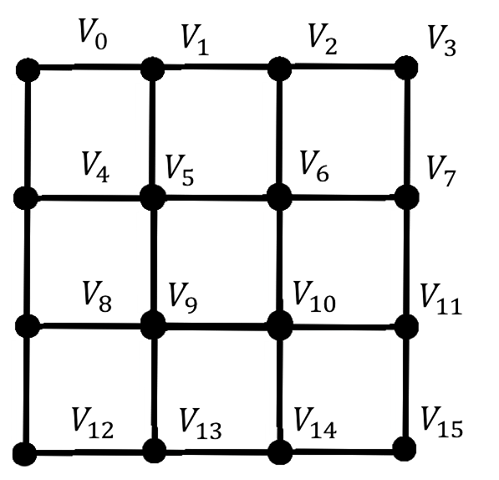
\includegraphics[width=0.3\textwidth]{4x4grid2.png}\label{gridFig}}
  \hfill
  \subfloat[]{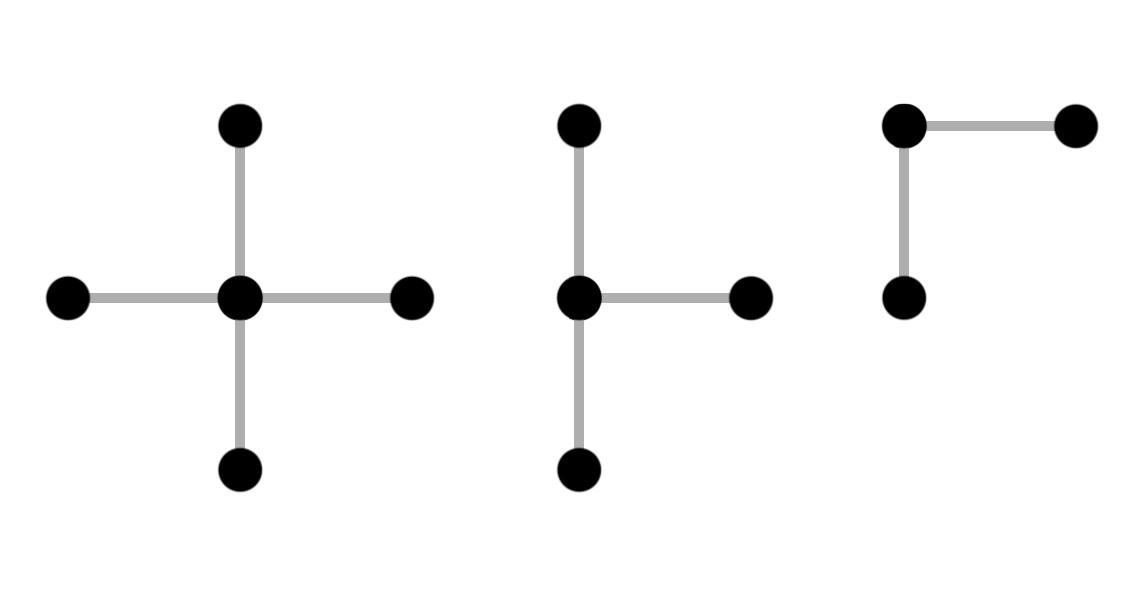
\includegraphics[width=0.5\textwidth]{stencils}\label{stencils}}
  \caption{(a)An example of a $4 \times 4$ grid. (b) Some incarnations of the 
stencil at various points on the grid}
\end{figure}

\begin{figure}[!h]
  \centering
\subfloat[]{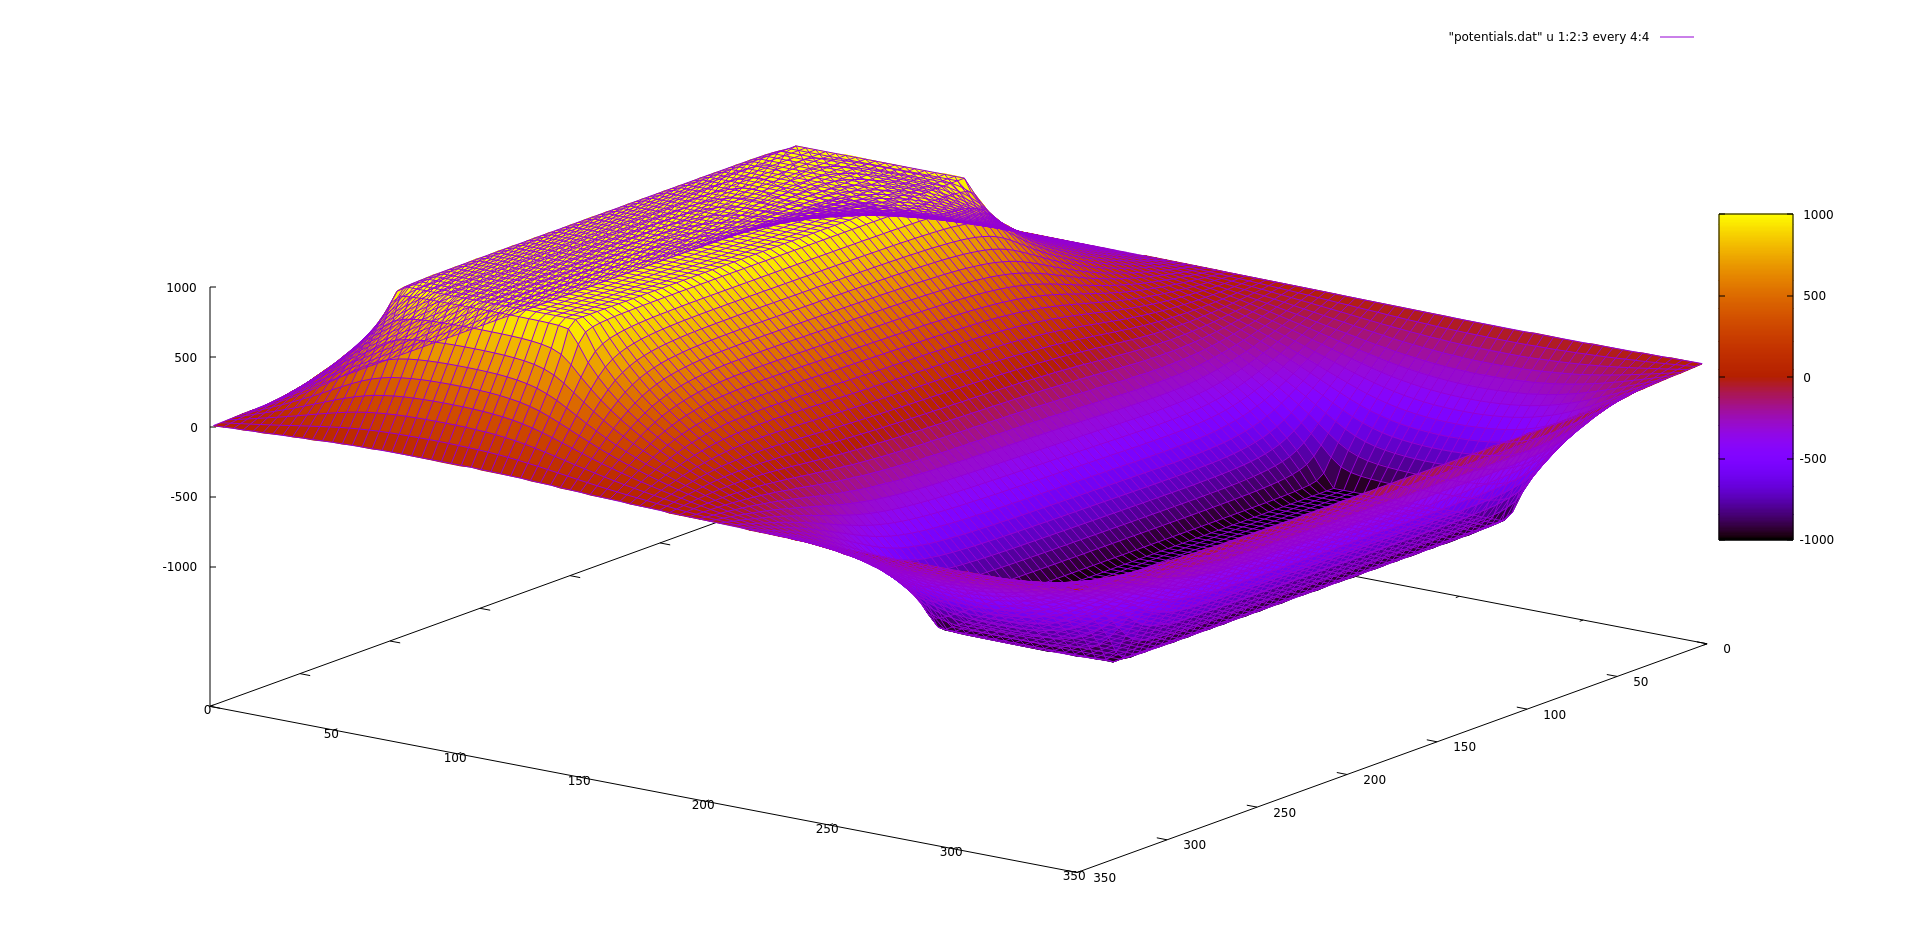
\includegraphics[width=0.5\textwidth]{fixedboundary}\label{fxbound}}\hfill
\subfloat[]{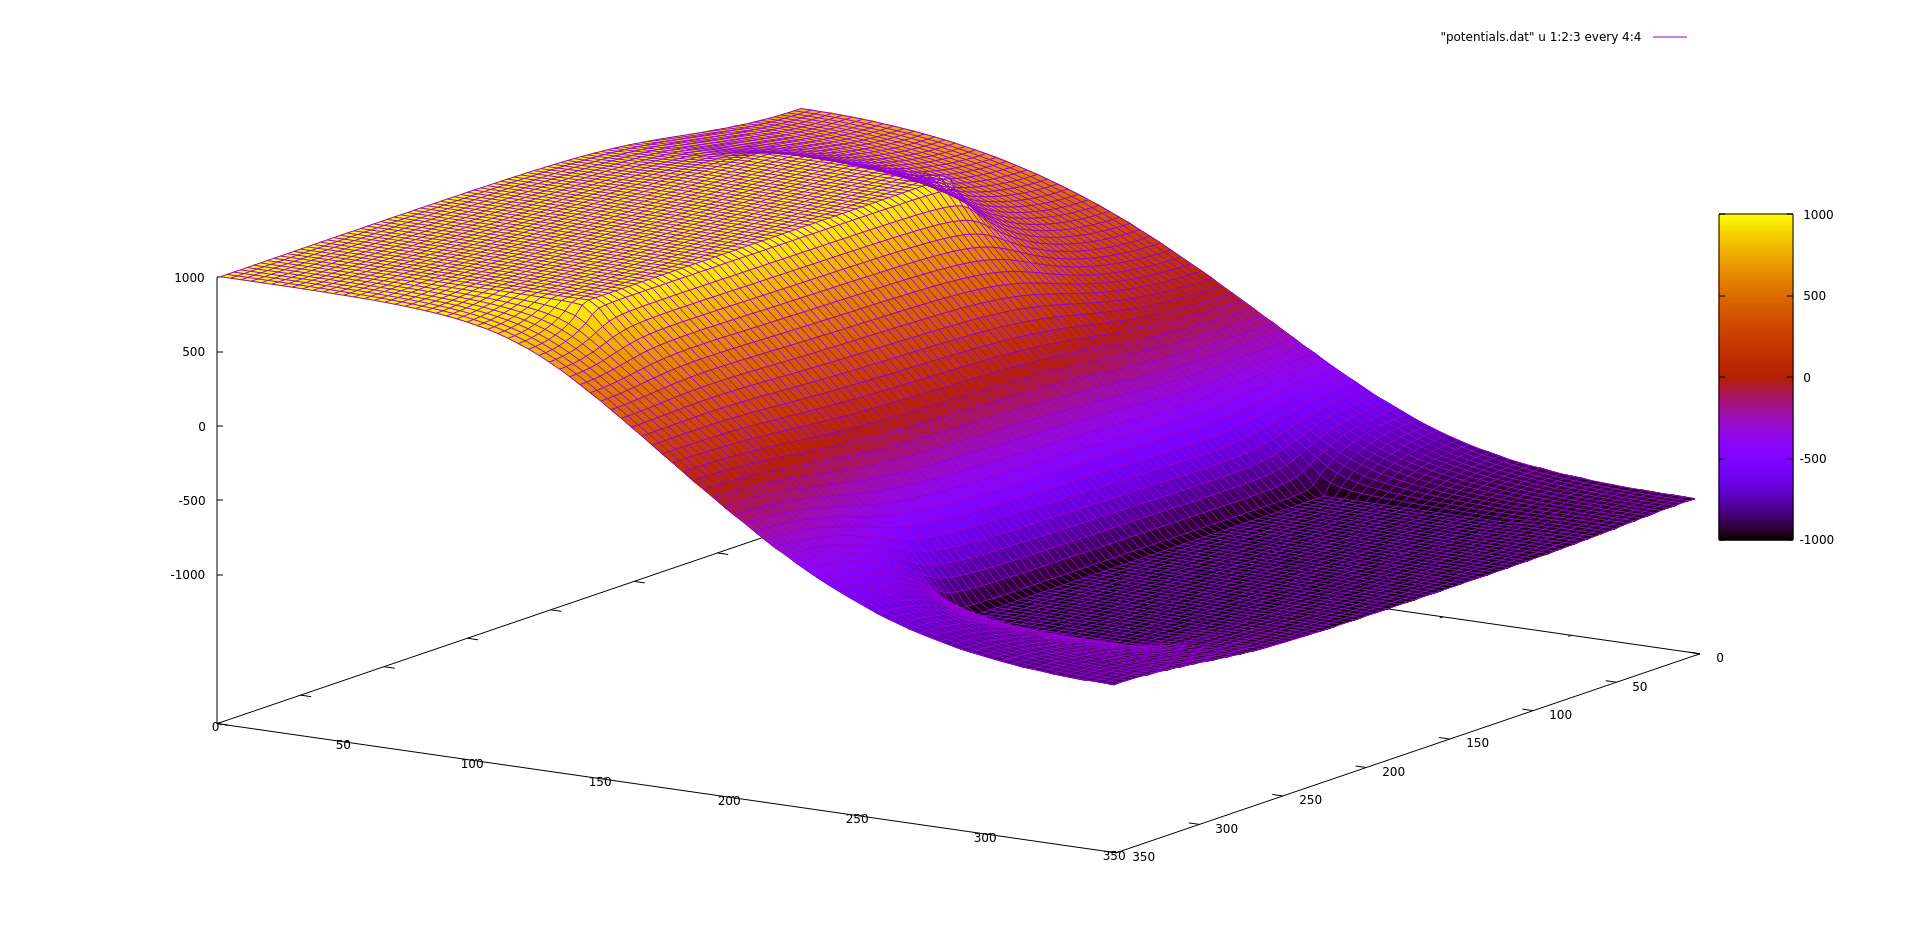
\includegraphics[width=0.5\textwidth]{adaptiveboundary}\hfill
\label{adbound}}
  \caption{Results with and without adaptive stencilling respectively. Notice 
how the boundaries are no longer fixed at zero.}
\end{figure}
\pagebreak
Now that the matrix can be stored and tailored to our problems we can explore
how the system is solved.

\subsection{Solving the Linear System}
Since taking full advantage of a CPU through efficient symbolic manipulation of
the matrices, and linking the algorithms to a specialised linear algebra
library is a very challenging task, we decided to utilise the SuperLU package
for solving.

To explain how SuperLU works we will break up the stages of the simplest
algorithm it employs to solve a Equation~\eqref{matEq}. The stage 1
concentrates on memory and the stage 2 on speed.

As mentioned earlier the matrix A is a very large, asymmetric and sparse  
matrix so we store it in CCS form. This however would pose a problem since 
computing simple LU decomposition would result in dense L and U matrices, 
instantly defeating the purpose of storing A in CCS format. This is treated by 
SuperLU in part 1 of the following algorithm called `Simple Driver Algorithm'
seen underneath.

Compute $P_rAP_c = LU$ where $P_r$ is a permutation matrix which reorders the 
rows and $P_c$ reorders the columns. $L$ is a unit lower triangular matrix and
$U$ an upper triangular one.
$P_c$ is chosen to order the columns of $L$ and $U$ to increase their sparsity. 
This is done by making use of another data structure called supernodes. 
Supernodes group together columns with the same non-zero structure thus 
conserving space. It makes sense then that to maximise the effectiveness of 
supernodes we permute the matrix to bring together columns with the same 
non-zero structures. This can be done without destroying important 
information by a post-ordering on $\mat{A}$'s column elimination tree \cite{ref27}
which is computed in time almost directly proportional to the number of
non-zero entries \cite{ref35}, giving us $P_c$. SuperLU can then perform
dynamic pivoting and row-interchanging to simultaneously find the LU
factorisation of $P_c$, $\mat{A}$ and $P_r$.

Equation~\eqref{matEq} can therefore be solved via
$X = \mat{A}^{-1}\vect{b}= (P_r^{-1}LUP_c^{-1})^{-1}\vect{b} =
P_c(U^{-1}(L^{-1}(P_r(B))))$
corresponding to a permutation of the rows of $\vect{b}$, followed by solving a
number of triangular systems equal to the entries in $\vect{b}$ by substitution.
Similarly, followed by solving the same number of triangular systems, to obtain
an answer for $\vect{v}$ without explicitly computing the inverse of $\mat{A}$.

\section{Performance of the Direct Method}
We evaluated various metrics to gauge the performance of the algorithm. First
we measured execution time with image size (see Fig.~\ref{sizetestFig}).
\begin{figure}
	\centering
	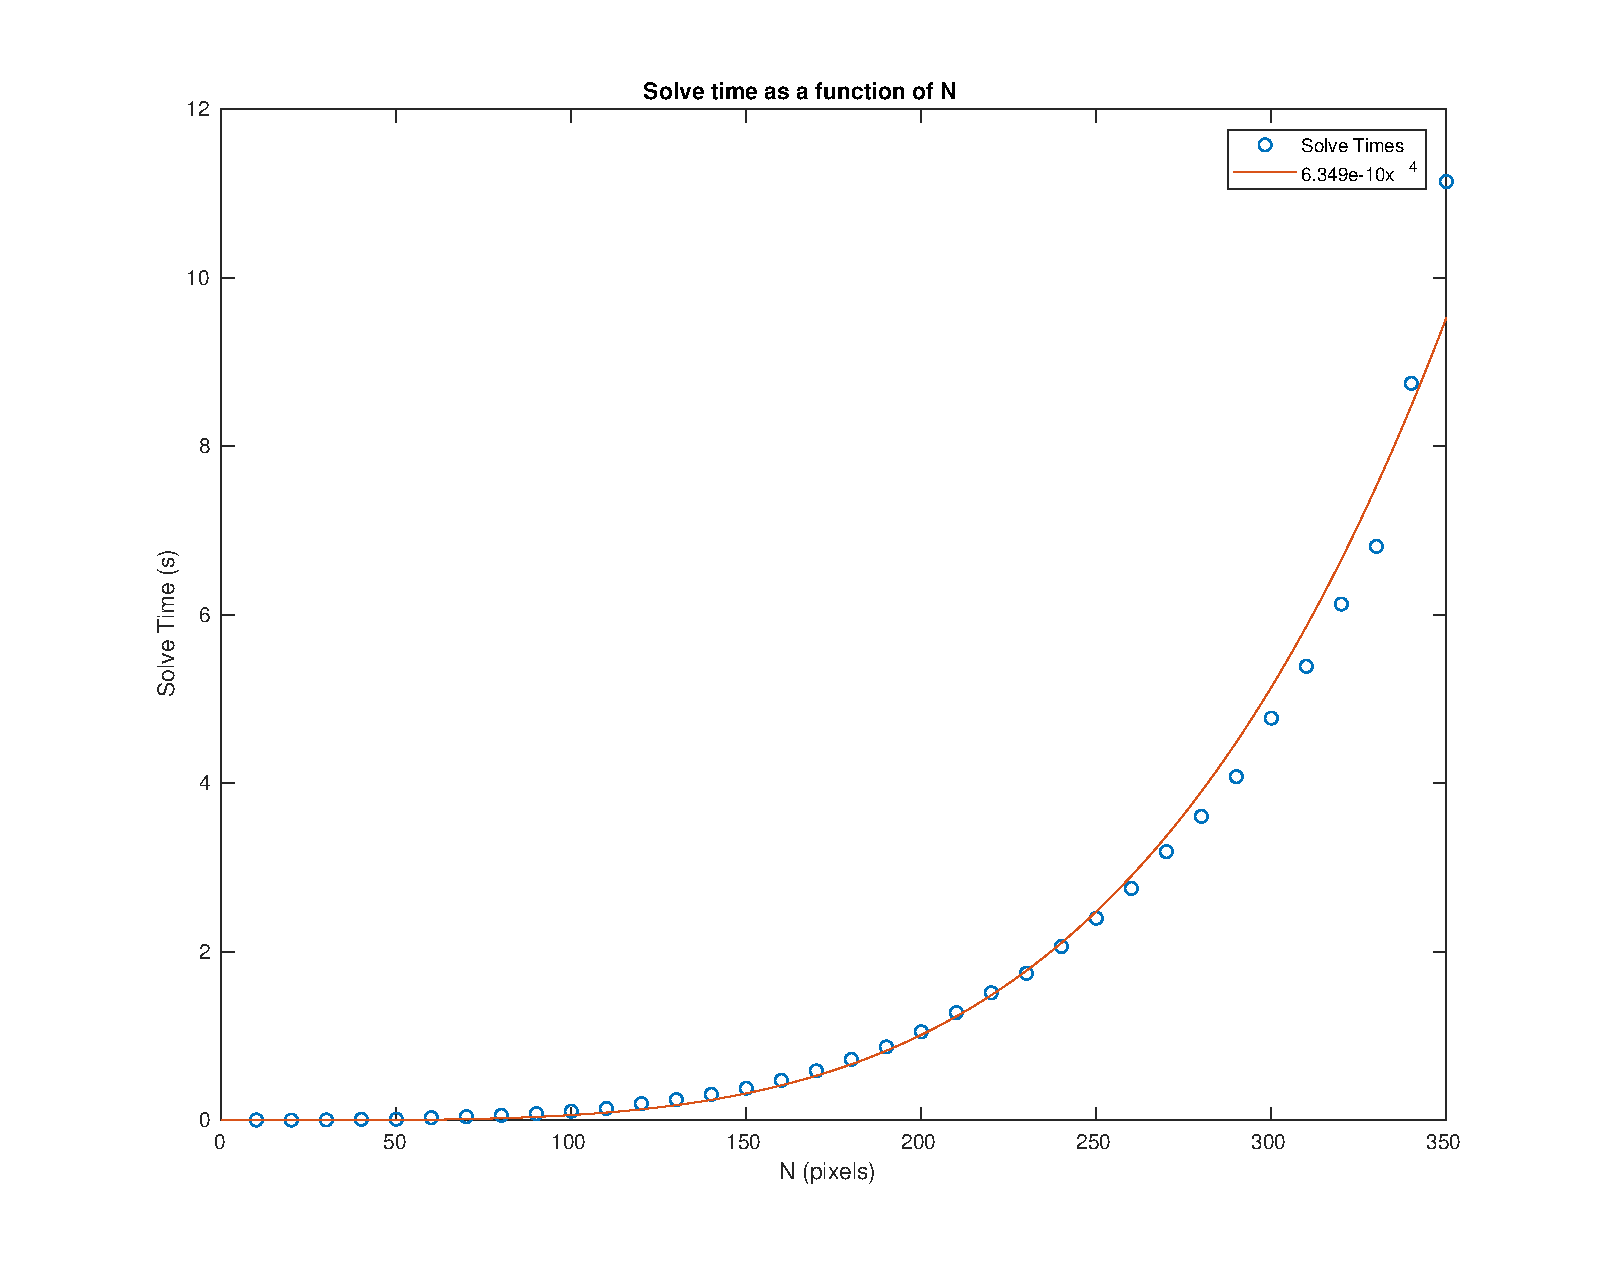
\includegraphics[scale=0.21]{sizebenchmark.eps}
	\caption{Variation of the solve time (in seconds) to $N$. The data fits
	quite well to a $N^4$ curve which is to be expected as this is the rate
	at which the matrix grows.}
	\label{sizetestFig}
\end{figure}
The code was tested with the same image at various sizes and the results were
plotted. Although exact solve times vary depending on the specific geometry,
the general trend should be the same.

Error was analysed by comparing the analytical results of Problem~0 and
Problem~1. For each pixel an absolute difference of the values was calculated
and we were able to use this to calculate the relative error of the numerical
solution.
        
%%%%%%%%%%%%%%%%%%%%%%%%%%%%%%%%%%%%%%%%%%%%%%%%%%%%%%%%%%%%%%%%%%%%%%%%%%%%%%%
%%%%%%%%%%%%%%%%%%%%%%%%%%%%%% PART 3 ANT %%%%%%%%%%%%%%%%%%%%%%%%%%%%%%%%%%%%%
%%%%%%%%%%%%%%%%%%%%%%%%%%%%%%%%%%%%%%%%%%%%%%%%%%%%%%%%%%%%%%%%%%%%%%%%%%%%%%%

\section{{\Large\textbf{Iterative Methods}}}
\subsection{Theory}\label{theory}
In this section, the Iterative Relaxation Method will be discussed, analysing 
its three different approaches: The Jacobi's Method, The Gauss-Seidel Method 
and the Successive Overrelaxation Method (SOR). 

The iterative methods rely on the fact that the Laplace Equation could be 
rewritten as a diffusive equation: \cite{NR}
\begin{equation}
\frac{\partial u}{\partial t}=\nabla^2u
\label{eq:Diffusion}
\end{equation}
Here $u$ defines potential, and the equation solved by this program is set in 
2D by assuming symmetry in the \textit{z} direction. It is important to note 
here that the Laplace equation is time independent by design, so the $t$ in 
equation \ref{eq:Diffusion} can be seen as introducing a fake time evolution
parameter. It is also evident from the equation that as the differential
$\frac{ \partial u}{\partial t}$ goes to 0, the solution for the Laplace
equation is reached. Now, using FTCS (Forward Time Centred Space) differencing,
the equation becomes \cite{NR}: 
\begin{equation}
u^{n+1}_{i,j}=u^n_{i,j}+\frac{\Delta 
t}{\Delta^2}(u^n_{i+1,j}+u^n_{i-1,j}+u^n_{i,j+1}+u^n_{i,j-1}-4u^n_{i,j})
\label{eq:FTCS}
\end{equation}
Where $\Delta ^2$ is the grid spacing in the \textit{x} or \textit{y} axis. 
This is the Jacobi equation, with the subscript \textit{n} denoting the 
simulated time evolution of the distribution $u$, while the terms $i$ and $j$ 
represent the real evolution in space along the two axes. This nomenclature 
describes how the iterative methods discussed in this report use the current 
point $u^{n}_{i,j}$ and its neighbouring points to affect the next point in the 
evolution $u^{n+1}_{i,j}$. Moreover, using Von Neumann stability analysis shows 
that the equation is stable if $\frac{\Delta t}{\Delta^2}<\frac{1}{4}$ when 
dealing with two dimensions in space \cite{matrixcomp} \cite{NR}.

We can make a slight improvement to the Jacobi method by introducing the 
Gauss-Seidel method which makes use of updated values of $u^n_{i,j}$ as soon as 
they become available:
\begin{equation}
u^{n+1}_{i,j}=u^n_{i,j}+\frac{\Delta 
t}{\Delta^2}(u^n_{i+1,j}+u^{n+1}_{i-1,j}+u^n_{i,j+1}+u^{n+1}_{i,j-1}-4u^n_{i,j})
\label{eq:Gauss}
\end{equation}
Finally, we introduce the Successive Overrelaxation Method (SOR): 
\begin{equation}
u^{n+1}_{i,j}=u^n_{i,j}+\frac{\Delta t}{\Delta^2} \omega 
(u^n_{i+1,j}+u^{n+1}_{i-1,j}+u^n_{i,j+1}+u^{n+1}_{i,j-1}-4u^n_{i,j})
\label{eq:SOR}
\end{equation}
The SOR method (\ref{eq:SOR}) introduces a relaxation parameter $\omega$ which 
makes an over correction to the value of $u^n_{i,j}$, de facto anticipating 
future corrections of the value. This over correction produce a considerable 
increase in the speed of the method. While the SOR method is convergent for 
$0<\omega<2$, we found that the only way to speed up the process is through 
overrelaxation, which occurs for: $1<\omega<2$. The optimal value of the 
overrelaxation parameter omega for a square grid is thus given by the 
expression\cite{omega} \cite{matrixcomp}:
\begin{equation}
\omega \approx \frac{2}{1+sin(\frac{\pi}{N})}
\label{eq:Omega}
\end{equation}
Where $N$ is the size of the square grid in one dimension

\subsection{Boundary Condition}
One of the most complex problems encountered during this project has been 
dealing with the grid's boundaries. The problem arises from the fact that all 
the methods discussed previously need four points in order to be successful, 
something which does not happen at the boundaries as only three (and two at the 
corners) points are available. Through literature readings we decided that the 
best method to be used was the \textit{Von Neumann Boundary Condition} 
\cite{vonNeumann}. The idea at the core of its method is to assume that close
to the boundaries the slopes between those points can be approximated to be
equal. If, for example, the left hand side boundary needs to be calculated,
then it is safe to say that 
$$\frac{u^n_{i,1}-u^n_{i,-1}}{2}=\frac{u^n_{i,3}-u^n_{i,1}}{2}=f'(u)$$
Where $u^n_{i,-1}$ is a \textit{ghost} point outside the grid.  Now, since
$u^n_{i,-1}=u^n_{i,1}-2f'(u)$, the point $u^n_{i,0}$ can be 
calculated as:
\begin{equation}
u^n_{i,0}=\frac{1}{4}(2u^n_{i,1}-2f'(u)+u^n_{i+1,0}+u^n_{i-1,0})
\label{eq:vonneumann}
\end{equation}
Equation \ref{eq:vonneumann} is used to calculate the points at the boundaries 
with the exception of the corner points.
\begin{equation}
u^n_{0,0}=\frac{1}{2}(u^n_{1,0}+u^n_{0,1})
\label{eq:corner}
\end{equation}
In order to get those point, for example for the upper left corner, we take an 
average of its two immediate neighbours, as described by equation 
\ref{eq:corner}.

\subsection{Results}
This section aims to discuss and compare the differences between the Jacobi, 
the Gauss-Seidel and the SOR method. To do this, we consider a 350$\times$350
PNG file depicting the layout of \ref{fig:nobel} as outputted by the GUI. The
boundary conditions of this problem are thus set to two parallel infinite
plates set to a voltage of $-1000$, enclosing a strip of centred grounded wire.
Updating the rest of the points iteratively using the three aforementioned
methods provided the following results.
\begin{figure}[!h]
  \centering
  \subfloat[]{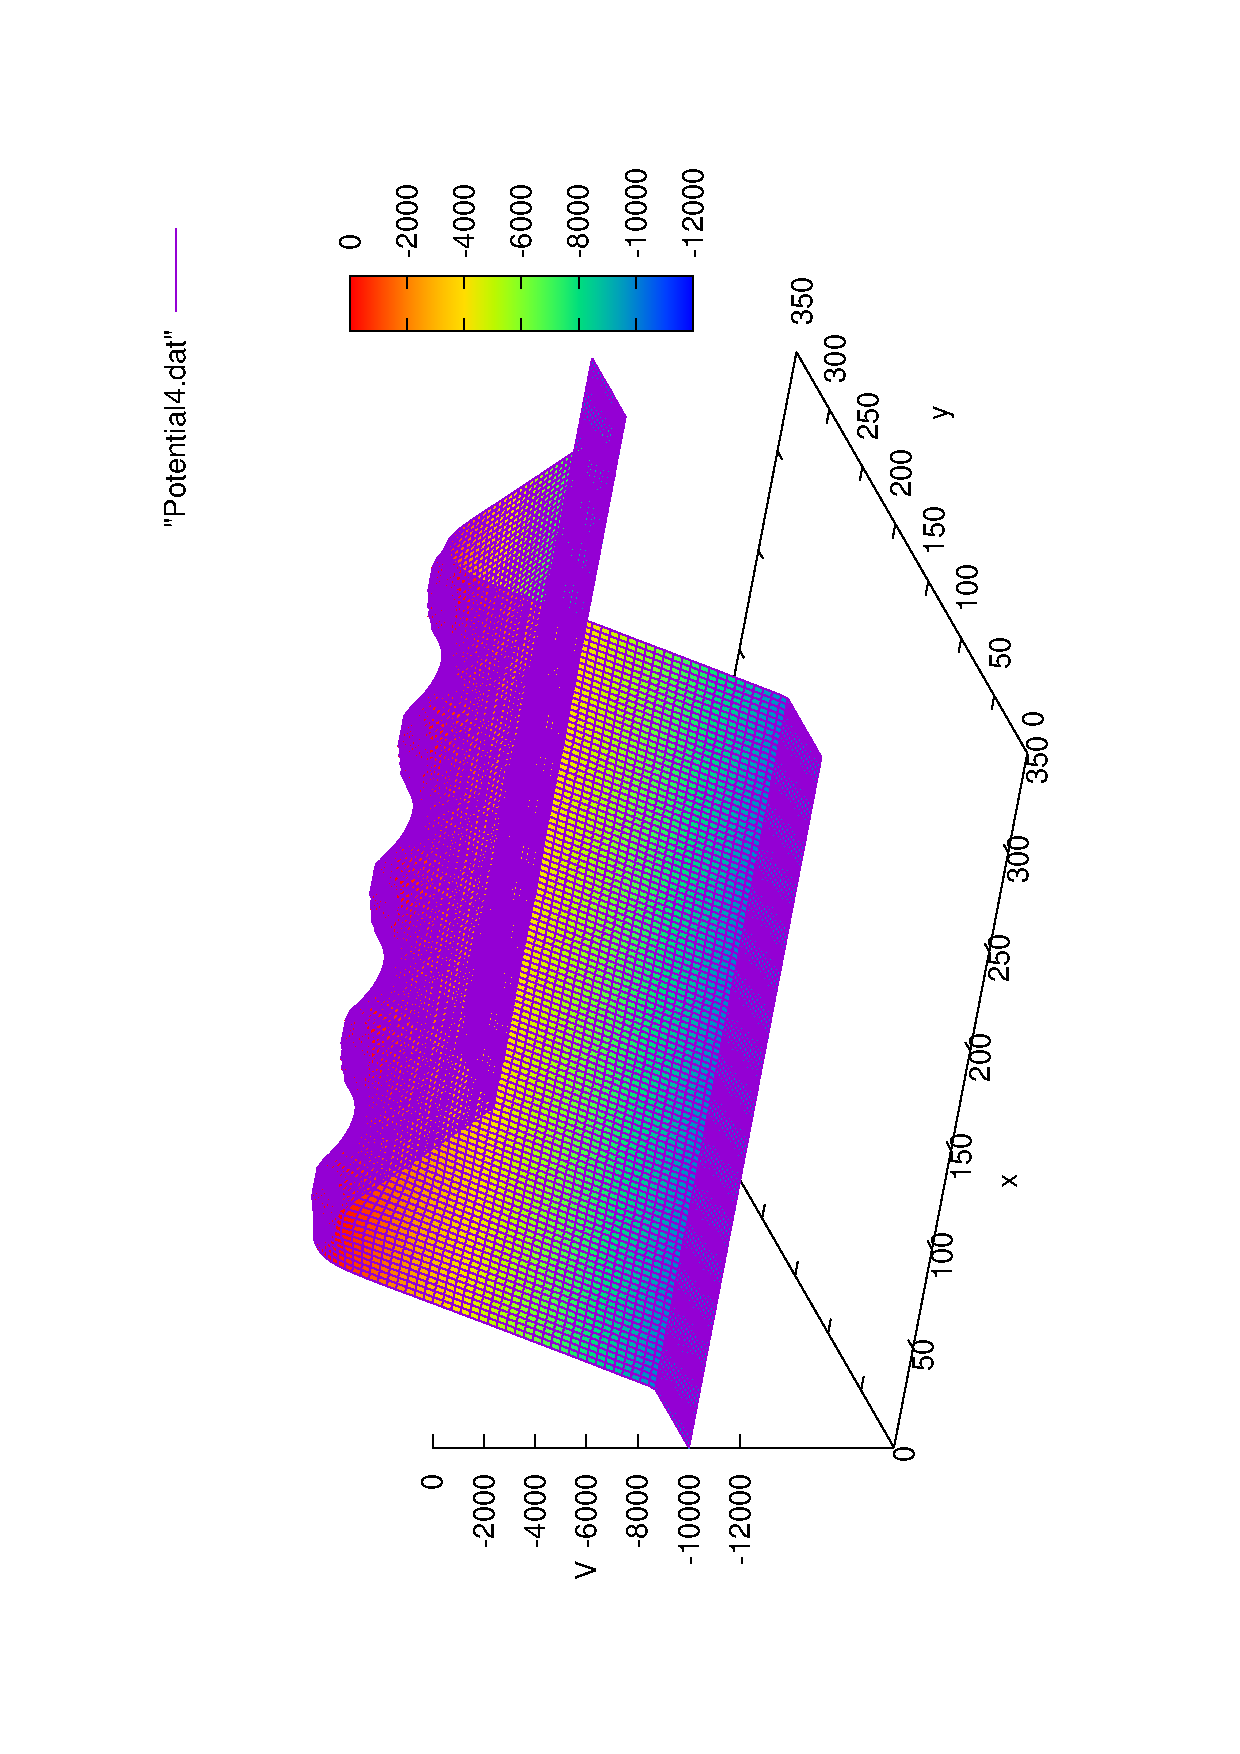
\includegraphics[width=0.4\textwidth, 
angle=-90]{Potential4}\label{fig:nobel}}
  \hfill
  \subfloat[]{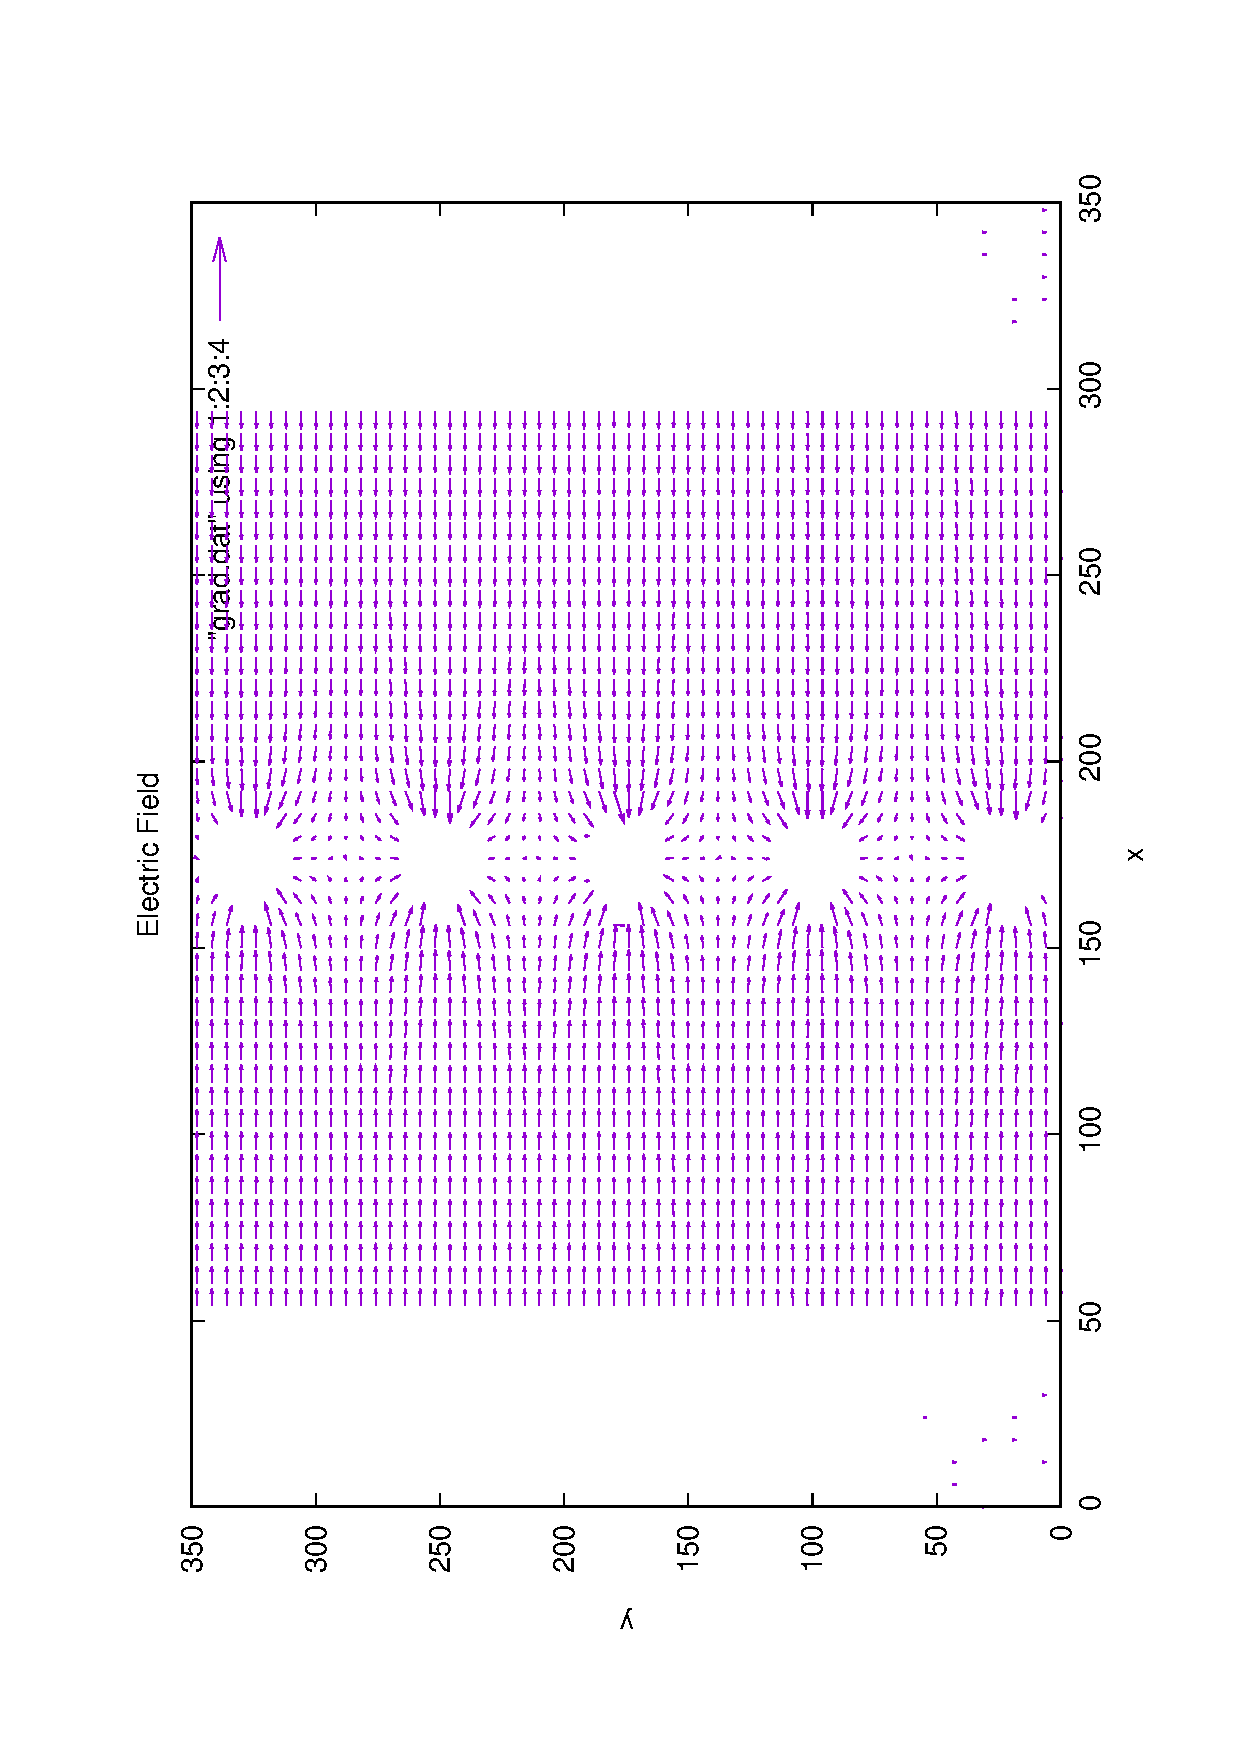
\includegraphics[width=0.3\textwidth, 
angle=-90]{grad}\label{fig:input}}
  \caption{The final version of the GUI, colour highlighted to aid with 
explanation.}
  \label{fig:results}
\end{figure}

\begin{table}[h!]
\centering
\begin{tabular}{| c | c | c | c |}
\hline
Method & CPU time (s) & Iterations & error tolerance\\
\hline\hline
$Jacobi's$ & $54.8108$ & $5915$ & $1 \times 10^{-2}$\\
\hline
$Gauss-Seidel$ & $40.7208$ & $4279$ & $1 \times 10^{-2}$\\
\hline
$SOR$ & $5.79559$ & 461 & $1 \times 10^{-2}$\\
\hline
\end{tabular}
\caption{Iterative Methods}
\label{table:methods}
\end{table}

Table \ref{table:methods} shows how the choice of the method affects the time 
taken by the program to produce solution as shown in figure \ref{fig:results}. 
We note here that what is considered to be an `acceptable solution' is quantified 
by the user defined error tolerance, which triggers a stopping mechanism that 
will be discussed later in the report.Table \ref{table:methods} shows how the 
choice of the method affects the time taken by the program to produce an 
acceptable solution as shown in figure \ref{fig:results}. It is clear from 
table \ref{table:methods} that the SOR method is indeed the fastest method 
among the ones discussed in section \ref{theory}. Moreover, we can see that the 
relaxation parameter allows us to get to the same solution produced by the 
other methods with a considerably less number of iterations, thus requiring 
significantly less computation time.

In section \ref{theory} it has been discussed how the SOR method depends on the 
overrelaxation factor $\omega$. If equation \ref{eq:Omega} is applied to the 
350$\times$350 grid mentioned before, we get the following result for the optimal 
factor: $\omega \approx 1.98221$. A simple plot of computational time versus 
applied $\omega$ shown in \ref{fig:omega} confirms that the optimal value of 
$\omega$ indeed lies in the immediate neighbourhood of  $1.98221$.
Figure \ref{fig:omega} confirms that the optimal value of $\omega$ lies in the 
immediate neighbourhood of  $1.98221$, and, as a consequence, so is equation 
\ref{eq:Omega}. 
\begin{figure}[h!]
\centering
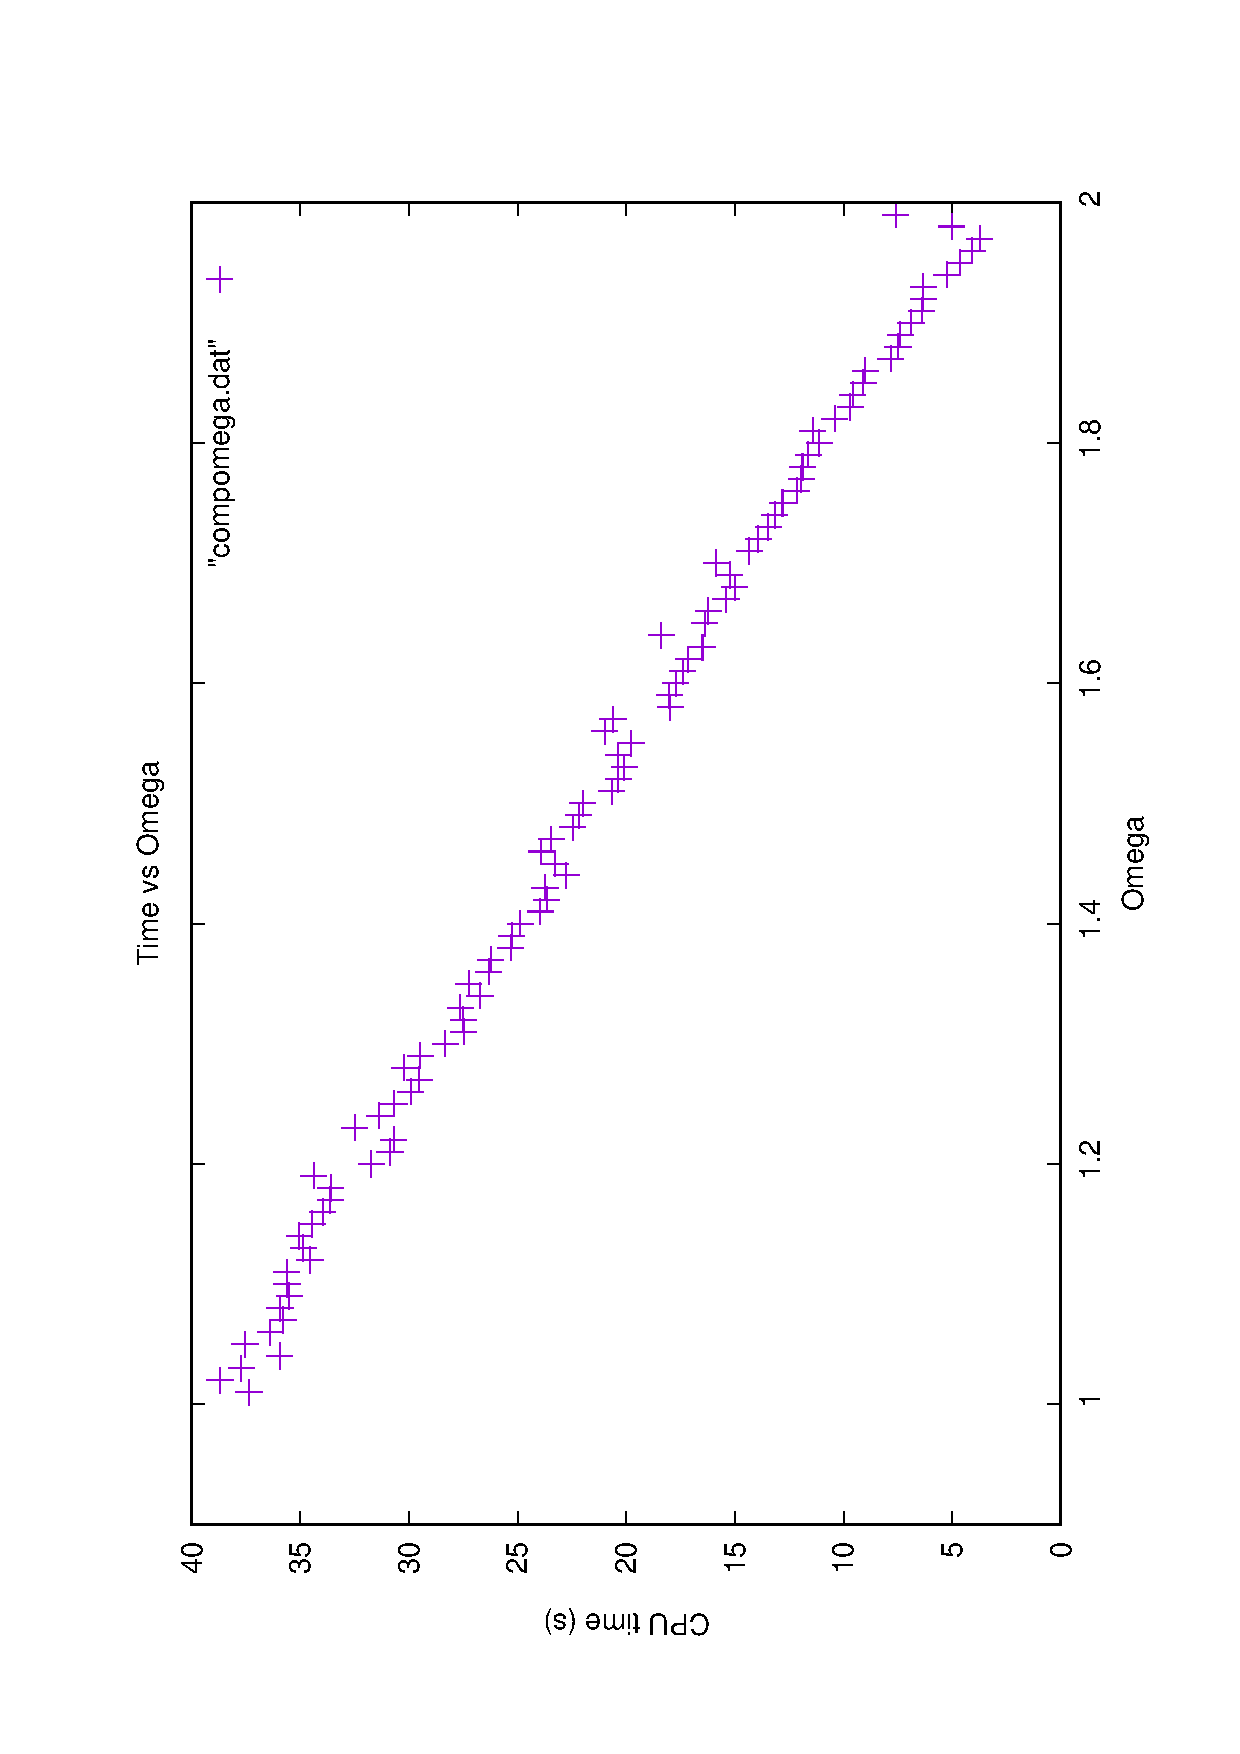
\includegraphics[scale=0.35,angle=-90]{compomega}
\caption{$\omega$ against Time}
\label{fig:omega}
\end{figure}
Having chosen the optimal combination of iterative method and relaxation 
parameter, we now have another dependable method for simulating electrostatic 
problems. The following section will further illustrate the optimisations and 
limitations that have been done to achieve the best possible accuracy and 
computational time, as well as providing a comparison between the direct and 
iterative methods as a whole.

%%%%%%%%%%%%%%%%%%%%%%%%%%%%%% PART 4 NIK %%%%%%%%%%%%%%%%%%%%%%%%%%%%%%%%%%%%%

\section{Optimisations, Errors and Comparisons}
Having discussed the inner workings of the iterative method, we can now 
consider the optimization and error analysis that the code underwent. In 
particular, we tackle boundary inaccuracies with different combinations of 
different approaches, as well as a stopping mechanism which gives the GUI user 
control of the iterative method. Lastly an error analysis is presented by 
comparing Direct and Iterative schemes with themselves and the analytical 
results. 
    
\section{The Boundary Problem}
As previously explained, the finite difference schemes obtain their values by 
considering the neighbouring points, with the boundary condition points 
remaining fixed. However, this also fixes all the edges to 0 which yields 
unphysical solutions  of `bounded free space' with often sharp slopes forced to 
zero as shown in Figure \ref{fig:boundprob}
\begin{figure}[!h]
  \centering
  
\subfloat[]{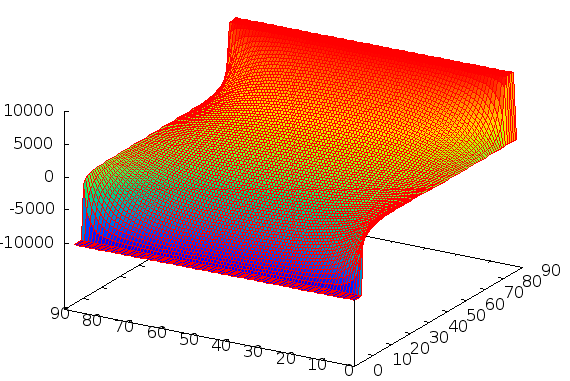
\includegraphics[width=0.4\textwidth]{noboundaries}\label{fig:GUI}}\hfill
  \subfloat[]{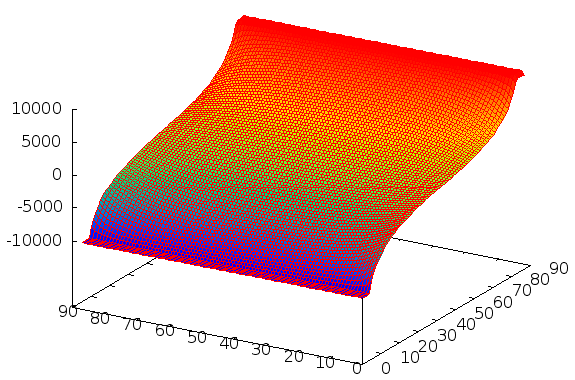
\includegraphics[width=0.4\textwidth]{noboundariesbigcanvas}\label{f ig:input}}\hfill
  \caption{Demonstrating the problem of bounded boundaries and a solution using 
concentric canvases}
  \label{fig:boundprob}
\end{figure}
There are two ways to address this issue as we check for how they work
individually and in tandem. Namely we can apply the previously discussed von 
Neumann boundary conditions, and the method of concentric canvases. The latter 
method in particular was improvised, and will thus have it's workings 
elaborated further below.

\subsection{Concentric Canvases}
In order to simulate a natural boundary behaviour for any geometry we introduce 
a bigger canvas A, concentric with our area of interest canvas B, as shown in 
Figure \ref{fig:canv}. By applying the boundary conditions on the bigger canvas 
we minimize the error effect on the simulated area with the assumption that 
potentials will tend towards zero at large distances in an attempt to simulate the effects of infinite space. \\

\begin{figure}[!h]
  \centering
  
\subfloat[]{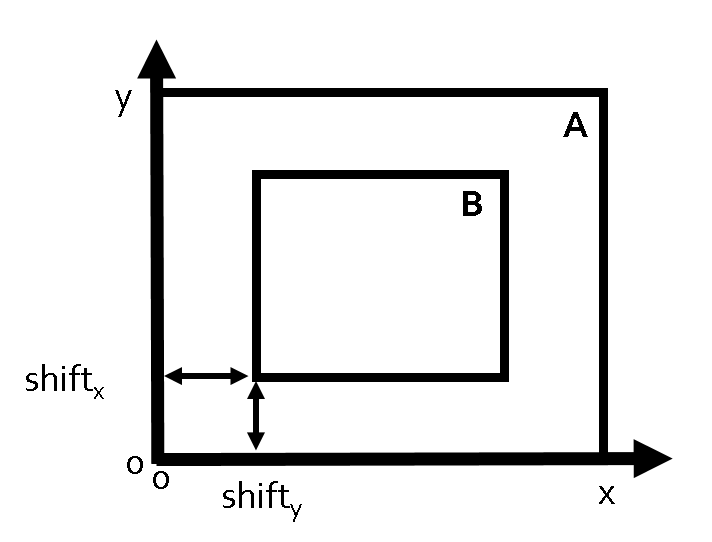
\includegraphics[width=0.4\textwidth]{concentriccanvases}\label{fig:
GUI}}
  \hfill
  \subfloat[]{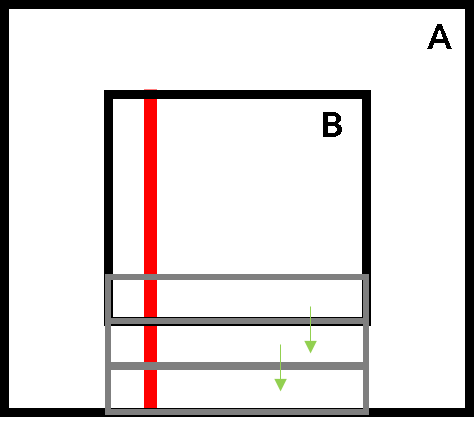
\includegraphics[width=0.3\textwidth]{Picture1}\label{fig:input}}
  \caption{Concentric canvases A and B with B the area of interest(left), 
Infinite Mode methodology; duplicating boundary of canvas B to the edge of 
canvas A (right)}
\label{fig:canv}
\end{figure}

\subsubsection{Simulating Infinite Plates}
Although this approach successfully simulates finite geometries, it fails to 
simulate scenarios of infinite plates since plates that span the small canvas 
B, are effectively finite in respect to canvas A. However, here we can take 
advantage of the bigger canvas A.

This is possible to do by extending the plate from canvas B to the edges 
of canvas A. This is done by simply duplicating the boarders of canvas B to the 
edges of canvas A as shown in Figure \ref{fig:canv} but still plotting 
potentials within canvas B. The result is to eliminate gradient components out 
or towards the canvas, parallel to the two plates as show in Figure 
\ref{fig:efield}

\begin{figure}[!h]
  \centering
  \subfloat[]{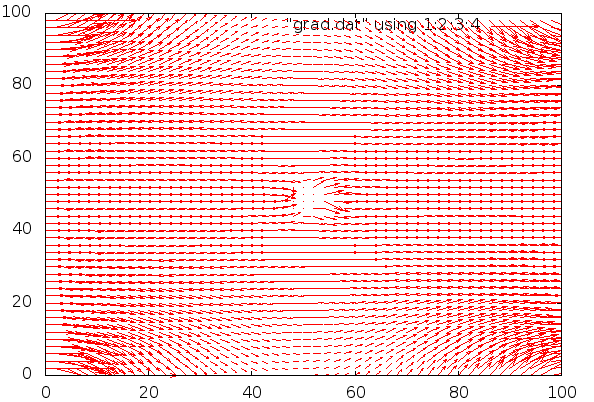
\includegraphics[width=0.4\textwidth]{infiniteon}\label{fig:GUI}}\hfill
\subfloat[]{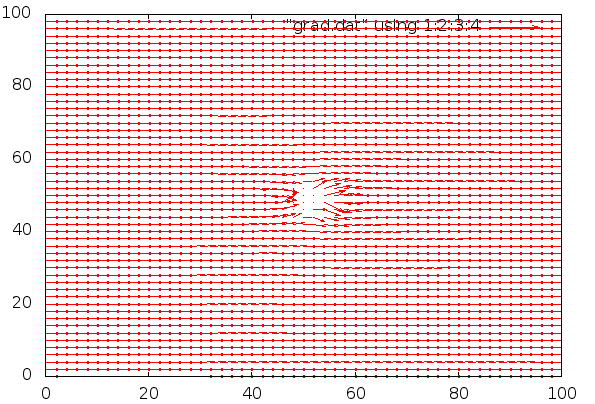
\includegraphics[width=0.4\textwidth]{infiniteoff}\label{fig:input}}\hfill
  \caption{Plotting the vector field \textbf{E} without and with Infinite Mode.}
\label{fig:efield}
\end{figure}

\com{\begin{figure}[h]
\centering
\begin{subfigure}{0.3\textwidth}
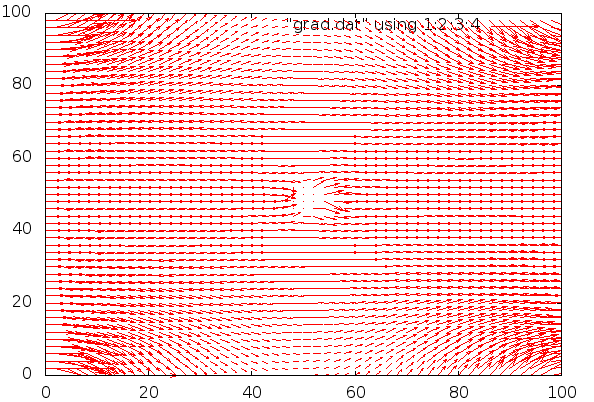
\includegraphics[width=\textwidth]{infiniteon}
\end{subfigure}
\quad
\begin{subfigure}{0.3\textwidth}
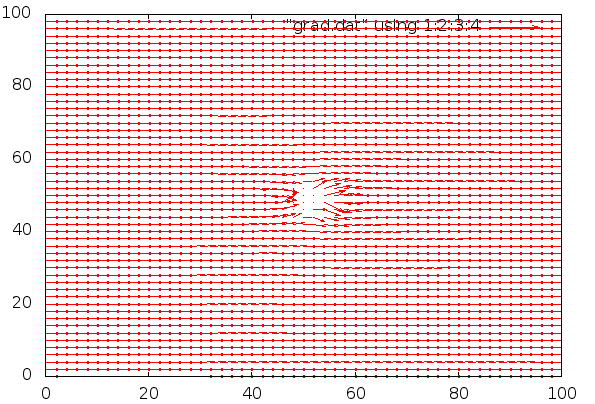
\includegraphics[width=\textwidth]{infiniteoff}
\end{subfigure}
\caption[Optional caption for list of figures 5-8]{Plotting the vector field 
\textbf{E} without and with Infinite Mode.}
\label{fig:efield}
\end{figure}}


\subsubsection{Optimum Canvas Size}
However, we should carefully choose a canvas size since it heavily affects 
computational speed, requiring more iterations to solve. Below we can see 
computational time to be proportional to $N^2$ for the canvas size we are 
solving. By considering again Problem 1 and its analytical answer, the 
relative error is plotted against different canvas ratios. Complimentary to 
that, Figure 1.4 shows both iterations and computational time to reach a 
certain relative error against different canvas ratios. As expected a bigger 
canvas ratio is computationally heavier, but more accurate. Any canvas ratio
between 1.2 to 1.5 provides increasing accuracy with a relatively small time
cost. We finally found the preferred size to be n=1.2, followed by further
analysis on the combination of this approach and boundary conditions. 
\begin{figure}[!h]
  \centering
  \subfloat[]{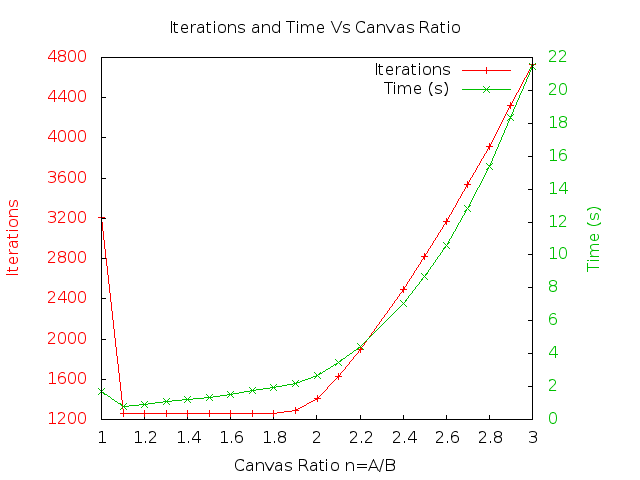
\includegraphics[width=0.5\textwidth]{time}\label{fig:GUI}}
  \hfill
  \subfloat[]{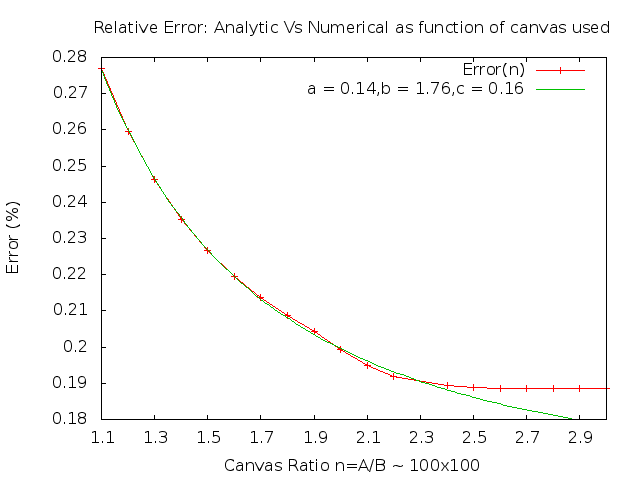
\includegraphics[width=0.5\textwidth]{percerror}\label{fig:input}}
  \caption{Plotting Iterations and Computational Time against different canvas 
sizes as well as the relative error compared to the analytical results for 
Problem 1. }
\label{fig:optcanv}
\end{figure}

\section{Combined Results}
It is in our interest to examine the combination of the two methods considering 
Problem 1, by comparing our results with the analytical ones for. As 
shown in the table below, both methods, concentric canvases and von Neumann 
Boundary conditions improve the accuracy of the scheme. However it is clear 
that the latter drastically do so with significant improvement. Specifically 
the best combination was using a canvas of ratio 1.2 with von Neumann Boundary 
conditions. Although there is a minuscule difference by using the `Infinite 
Mode', keeping it is motivated when the iterative method is compared with the 
direct method which will be discussed later.  
\begin{table}[h]
\centering
\begin{tabular}{c c c | c}
Boundary Cond. & Canvas Ratio (n) & Inf. Mode & Error(\%) \\
\hline
off & 1 & off & 26.75\\
 on & 1 & off & 0.81\\
off & 1.2 & off & 15.19\\
off & 1.2 & on & 13.44\\
on & 1.2 & on & 0.85 \\
on & 1.2 & off & 0.74 \\
\end{tabular}
\end{table}

\section{Stopping Mechanism}
As it comes to the optimization of our program,
It is important to have some control over the iterative method and what any 
particular user considers to be acceptable accuracy. Hence, we introduce a 
stopping mechanism as well as a maximum allowed iterations to prevent 
unreasonable long run times.\\

Since SOR method is a linear convergent method it can be shown that it 
satisfies the inequality 
\begin{equation}
\frac{\|u^{n+1}-u^{n} \|}{\|u^{n}-u^{n-1}\|} \approx r, \ \ \ r < 1
\end{equation}
where `n' is the `$n^{th}$' iteration and `r' the constant the ratio presented 
converges to.\cite{stop}
By assuming the forward in time solution, `$u^{n+1}$' to be an approximation to 
the true solution of the Laplace equation the relative error can be calculated. 
\begin{equation}
\frac{r}{1-r} \frac{\|u^{n+1}-u^{n} \|}{\|u^{n+1}\|} = \epsilon_{tol}
\end{equation}
where `$\epsilon_{tol}$' is the desired tolerance. `r' was calculated to be 
$0.996$. 

\section{Error}
\subsection{Comparison of Methods: Direct Vs Iterative}
By now, Emission has developed two separate methods for solving the Nobel Prize 
winning problem. It is then in our interest to compare the performance of 
the two methods with regards to the Nobel Prize Problem. Since the iterative 
method by definition converges to the direct method, the latter is used as the 
reference for calculating the relative error. 

\begin{table}[h]
\centering
\begin{tabular}{c c c c c c}
Boundary Cond. & Canvas Ratio (n) & Infinite Mode & Error(\%) & Iteration &  
Time\\
\hline
on & 1.2 & on & 0.718 & 468 & 6.69 \\
on & 1.2 & off & 0.518 & 458 & 6.76 \\
on & 1 & - &  0.075 & 460 & 4.48\\
\end{tabular}
\end{table}
It turns out that completely omitting the concentric canvas method yields the 
greatest agreement between the two methods (With a difference in order of 
magnitude by 1). This is expected since they are calculated in exactly the same 
manner as the direct method does not involve a larger canvas. That is, there 
are only relatively small errors mainly near the grounded circles themselves 
which are expected to decrease if the method is allowed to iterate more. 
Furthermore, one can argue that even with a concentric canvas, the results turn 
out to be in greater disagreement with the infinite mode activated rather than 
without it. However, as shown in Figure \ref{fig:iterVsdir}, on the first graph 
starting from left, the error is much less at the boundaries. That is the 
method is forces the boundaries to converge at a straight line faster.  

\begin{figure}[!h]
  \centering
  \subfloat[]{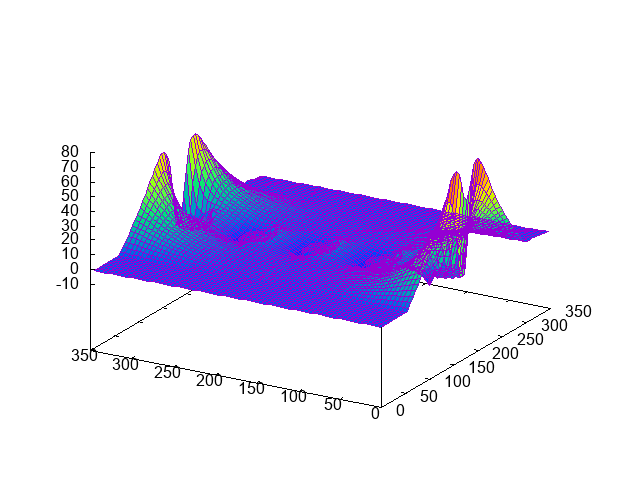
\includegraphics[width=0.3\textwidth]{c12wbinfon}\label{fig:GUI}}\hfill
\subfloat[]{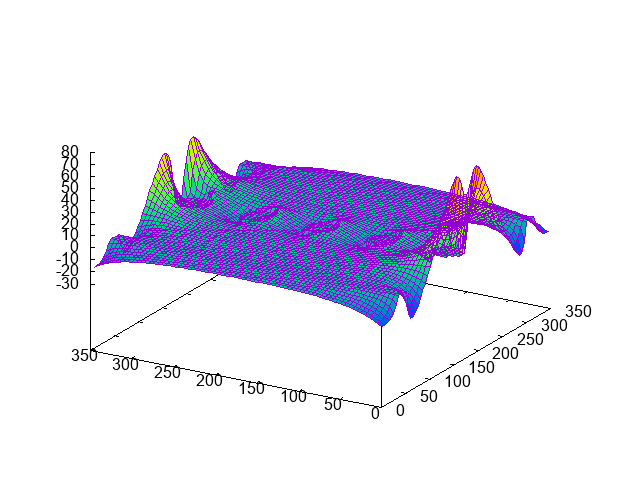
\includegraphics[width=0.3\textwidth]{c12wbinfoff}\label{fig:input}}\hfill
\subfloat[]{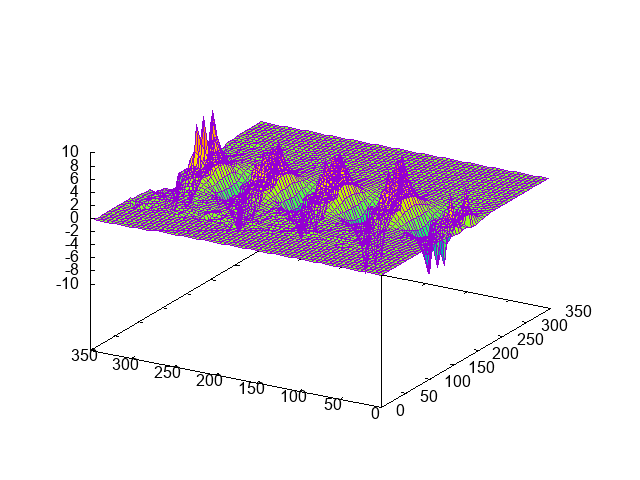
\includegraphics[width=0.3\textwidth]{c1wbinfoff}\label{fig:input}}\hfill
  \caption{Plotting the differences of 
Iterative and Direct Method. The graphs follows from left to right the 
tabulated order.}
  \label{fig:iterVsdir}
\end{figure}

Lastly, choosing the iterative method with combined concentric canvases 
approach and von Neumann Boundary conditions as the most general version we 
investigate the execution times of both methods on tackling problems 0, 1. The 
results are presented in the following tables. 

\begin{table}[h!]
\centering
\begin{tabular}{c | c c }
\textbf{Method} & \textbf{Execution Time} (s) & \textbf{CPU Memory}\\
\hline
\textbf{Iterative (SOR)} &  11.55911 & - \\
\textbf{Direct} & 8.6835   &  705.83\\
\end{tabular}
\caption{Problem 0}
\end{table}

\begin{table}[h!]
\centering
\begin{tabular}{c | c c }
\textbf{Method} & \textbf{Execution Time (s)} & \textbf{CPU Memory}\\
\hline
\textbf{Iterative (SOR)} &  20.3519 & - \\
\textbf{Direct} & 15.1301  & 1059.96\\
\end{tabular}
\caption{Problem 1}
\end{table}
In conclusion, both methods are developed and optimized to a great flexibility, 
able to solve any given, finite or infinite plate geometries. However, the 
iterative method is slightly more time inefficient, but offers more control 
to the user through the stopping mechanism, which can be toggled to low 
tolerance allowing us to obtain quick estimations or general trends.


%%%%%%%%%%%%%%%%%%%%%%%%%%%%%% PART 5 TOM %%%%%%%%%%%%%%%%%%%%%%%%%%%%%%%%%%%%%

\section*{The Graphical User Interface (GUI)}

The Emission project had always been intended to run using a GUI front end, 
allowing the user to have full control over the geometry and charge of the 
input potential. The following section of the report will document the 
development of such an interface, discussing the choice of development platform 
as well as the functionality of the final product.


\subsection*{Functionality}

At its core, the main purpose of a GUI is to provide an intuitive environment 
in which information necessary for solving a given problem can be extracted 
from the user. Given the fact that the problem this software package aims to 
solve is quite particular, it was important to lay out explicitly what 
information was needed from the user, as well as the methods used to 
communicate it.


As seen in the previous sections, both the direct and the iterative methods 
work by first reconstructing an image of arbitrary geometry, in which shapes 
and their colour provide boundary conditions for solving the potential field. 
Hence, the main purpose of the GUI had always been to provide the user with an 
image generator in which one can dynamically draw basic shapes of charge, 
specified by colours in a user defined spectrum. This setup allows for notable 
optimization by having the GUI output images at computationally manageable 
sizes, tailored to include only separate shades of green and red for different 
charges (this heavily simplifies the translational algorithm). All this while 
not depriving the user of the freedom to create any desired 2D boundary 
conditions.

Apart from a dynamic canvas, it was essential that we have a GUI that is fully 
integrated into the project framework. What this means is that the GUI can run 
alongside the two methods in a single executable, with the ability to store and 
pass variables of any type, which can then be used as input arguments to 
functions solving the problem. 

\subsection*{Developer Software}
%\begin{wrapfigure}{r}{0.43\textwidth}
%  \centering
%  {
\includegraphics[width=0.15\textwidth]{QtPic}\label{fig:Qt}}
%  \hfill
%\end{wrapfigure}
Having decided on the functionality of the GUI, the next step for us was to 
chose a developer platform which would allow us to create it within the given 
time frame. In the end, the GUI developing software chosen was Qt since it is 
geared towards C++ development which was our primary coding language. Moreover, 
Qt has its own project builder with a static compiler, allowing us to 
distribute the final product of Emission as a small Linux application. All 
this, coupled with comprehensive documentation for beginners made Qt a very 
ood choice and we could thus get started on building the GUI.

\subsection*{Implementation}

Building a GUI through Qt is inherently done through object orientated 
programming, as the entire framework is based on a hierarchy of classes and 
objects. Thus, we needed to define our own class which would act as a blueprint 
of all the things that make up what the user interacts with in the application 
window, which in turn would be the object. This blueprint would lay out all the 
data that the application needs to extract and store from the user, the visual 
layout, and the functionality. Moreover, we define our class to be a parent, 
inheriting other predefined Qt classes to widget objects such as buttons and 
pixmaps as its children. The final outcome is demonstrated by the figures 
below.

\begin{figure}[!h]
  \centering
  \subfloat[]{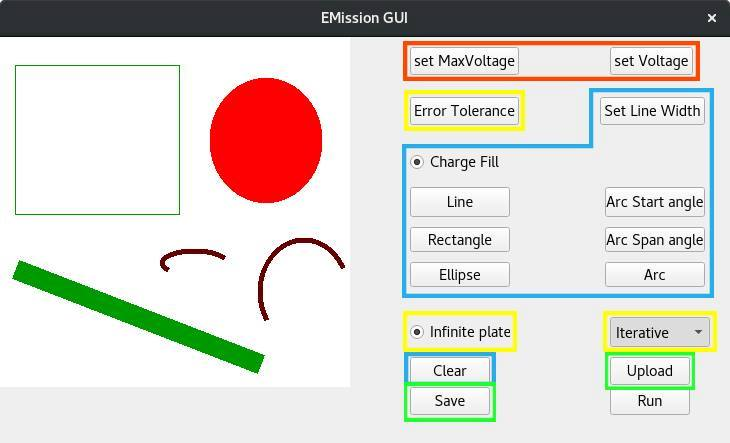
\includegraphics[width=0.62\textwidth]{GUI-demo}\label{fig:GUI}}
  \hfill
  \subfloat[]{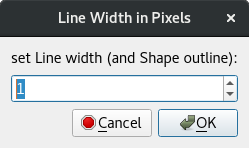
\includegraphics[width=0.32\textwidth]{input}\label{fig:input}}
  \caption{The final version of the GUI, colour highlighted to aid with 
explanation.}
\end{figure}


The first feature to point out is the voltage feature (red) which is integral 
in the translational algorithm. The user is given two input buttons which lead 
to a menu similar to the one projected in picture (b); there, the user sets an 
integer maximum voltage $x$, which allows us to assign a voltage to all the 
possible shades of red from $[0,x]$ as positive charges, and all possible 
shades of green  from $[-x,0]$ as negative charges. The user can then set a 
voltage from the second menu and draw with its respective colour, while the 
maximum voltage is stored and passed onto the solving algorithms.

The maximum voltage is then the first value stored by the program, and is of 
type integer. The next few variables that the program is storing are 
highlighted in yellow, and consist of a double value for the error tolerance at 
which the stopping mechanism of the iterative method activates; a boolean value 
which is toggled by a radio button, telling the program if the drawn geometry 
extends to infinity or not; and lastly a boolean  drop down menu allowing the 
user to choose between the iterative or direct method. Furthermore, green 
highlight points out functionality allowing the user to save their drawing into 
a gallery directory, or upload a picture of their liking by typing its file 
path. The file path of the picture chosen to be solved is saved as a string. 
Finally, the run button passes all this information as input to the solving 
functions which run Gnuplot internally.

The remaining functionality is highlighted in blue, and is demonstrated in the 
canvas of figure (a). First, we set the line width dialogue box to 1 pixel as 
shown in figure (b), and draw a rectangle with no fill at a negative voltage. 
Then, setting the voltage to be positive, we use the ellipse handle to draw a 
sphere with charge fill on. After this, the line width is set to 20 pixels, and 
voltage is changed back to negative as we draw a line which appears to be a 
diagonal rectangle. Finally, setting a relatively low positive voltage, we draw 
two arcs by first inputting their initial orientation with `start angle' and 
then the angle which they will span using `span angle'. The drawing is always 
done dynamically by selecting a shape and then clicking on the canvas, dragging 
to set the desired size, and then releasing. The clear function has also been 
included in case of an error.

The GUI described here is called as a function in the main program of the 
project, which allows for a segregation of Qt based programming from the rest of 
the project; the segregation thus only ever needs to be resolved through 
dependencies in the main header file. This type of compartmentalization is made 
possible thanks to the C feature of external programming which allows one 
script to access and overwrite variables of a different script, assuming that 
the two scripts are linked by the compiler. Hence, user keyboard and mouse 
interactions with the GUI can make real changes to input variables of the two 
solution methods, and Emission runs as a single compact unit. 

\section*{Conclusion}
The Emission Project has been developed with the intent to solve and simulate 
electrostatic problems of any geometry that can be described by the Laplace 
Equation.  To do this we have implemented two separate approaches of numerical
simulation in the form of direct and iterative methods. On comparing the two
methods, advantages and disadvantages became clear. The iterative methods were
found to be slower for a given relative error, perhaps partly due to the fact
that the routines written were almost completely written from scratch while the
direct method used heavily optimised libraries that linked to the Automatically
Tuned Linear Algebra Software (ATLAS) library. We implemented both Neumann and
Dirichlet boundary conditions and achieved relative error percentages on the
order of 1\%. Furthermore the methods agreed with a high degree of accuracy
with each other.  

In addition to this, we have ensured that the entire Emission project is 
presented as an application which can be run through a single executable, and 
has an integrated GUI allowing the user to freely create his or upload his own 
specific electrostatic geometries. Despite our progress, there are still 
notable areas of improvement for the code performance, including second order 
Von Neumann boundary conditions for the iterative methods, as well as 
simulation using multi gird methods which could drastically increase code 
performance. Nevertheless, we feel that Emission provides the user with a 
comprehensive and intuitive solver for general electrostatic problems.
The Emission project has been developed with the intent to solve and simulate 
electrostatic problems of any geometry.

\pagebreak
\bibliographystyle{alpha}
\begin{thebibliography}{15}

	\bibitem{NR}
		\emph{Numerical Recipes: The Art of Scientific Computing}\\
		W. H. Press, S. A. Teukolsky, W. T. Vetterling, B. P. Flannery\\
		September 2007\\
		ISBN: 9780521880688

	\bibitem{101matstore}
		\emph{101 Ways to Store a Sparse Matrix}\\
		Max Grossman\\
		\texttt{https://medium.com/@jmaxg3/101-ways-to-store-a-sparse
		-matrix-c7f2bf15a229}\\
		Accessed: 12\textsuperscript{th} March 2018
        
	\bibitem{matrixcomp}
		\emph{Fundamentals of matrix computations,  second edition}\\
		David S. Watkins\\
		2002

	\bibitem{omega}
		\emph{The optimal relaxation parameter for the SOR method
		applied to the Poisson equation in any space dimensions}\\
		Shiming Yang, Matthias K. Gobbert\\
		2008

	\bibitem{vonNeumann}
	\texttt{https://www.12000.org/my\_courses/UC\_davis/fall\_2010/math\_228a/HWs/HW3/Neumman\_BC\\
	/Neumman\_BC.htm}
            
	\bibitem{stop}
  		\verb!http://ta.twi.tudelft.nl/users/vuik/burgers/lin_notes.pdf!
  
	\bibitem{ref27} 
		\emph{R. Gilbert and E. Ng, Predicting structure in 
		nonsymmetric sparse matrix factorizations,
		in Graph Theory and Sparse Matrix Computation}\\
		A. George, J. R. Gilbert, and J. W. H. Liu, eds.,\\
		Springer–Verlag, New York, Berlin, 1993.
    
	\bibitem{ref35}
		\emph{The role of elimination trees in sparse factorization}
		J. W. H. Liu

	\bibitem{qtref}
		\emph{Qt Documentation}\\
		\texttt{http://doc.qt.io/qt-5/reference-overview.html}

	\bibitem{csparse}
		\texttt{
		https://github.com/PetterS/SuiteSparse/tree/master/CSparse 
		}
\end{thebibliography}
\end{document}
